% ==================================================
% Helper: appendix section shown as level-2 in TOC
% ==================================================
\newcommand{\appsection}[1]{%
    \refstepcounter{section}%
    \section*{Appendix \thesection: #1}%
    \addcontentsline{toc}{subsection}{%
        \protect\numberline{\thesection}#1%
    }%
}

% ==================================================
% Appendix A: RSI Landscape
% ==================================================
\pagestyle{appendixAstyle}

\appsection{RSI Landscape}
\label{app:rsi-landscape}

Figure~\ref{fig:rsi-landscape} summarizes the surveyed papers by autonomy level and improvement target.

\begin{figure}[!htbp]
    \centering
    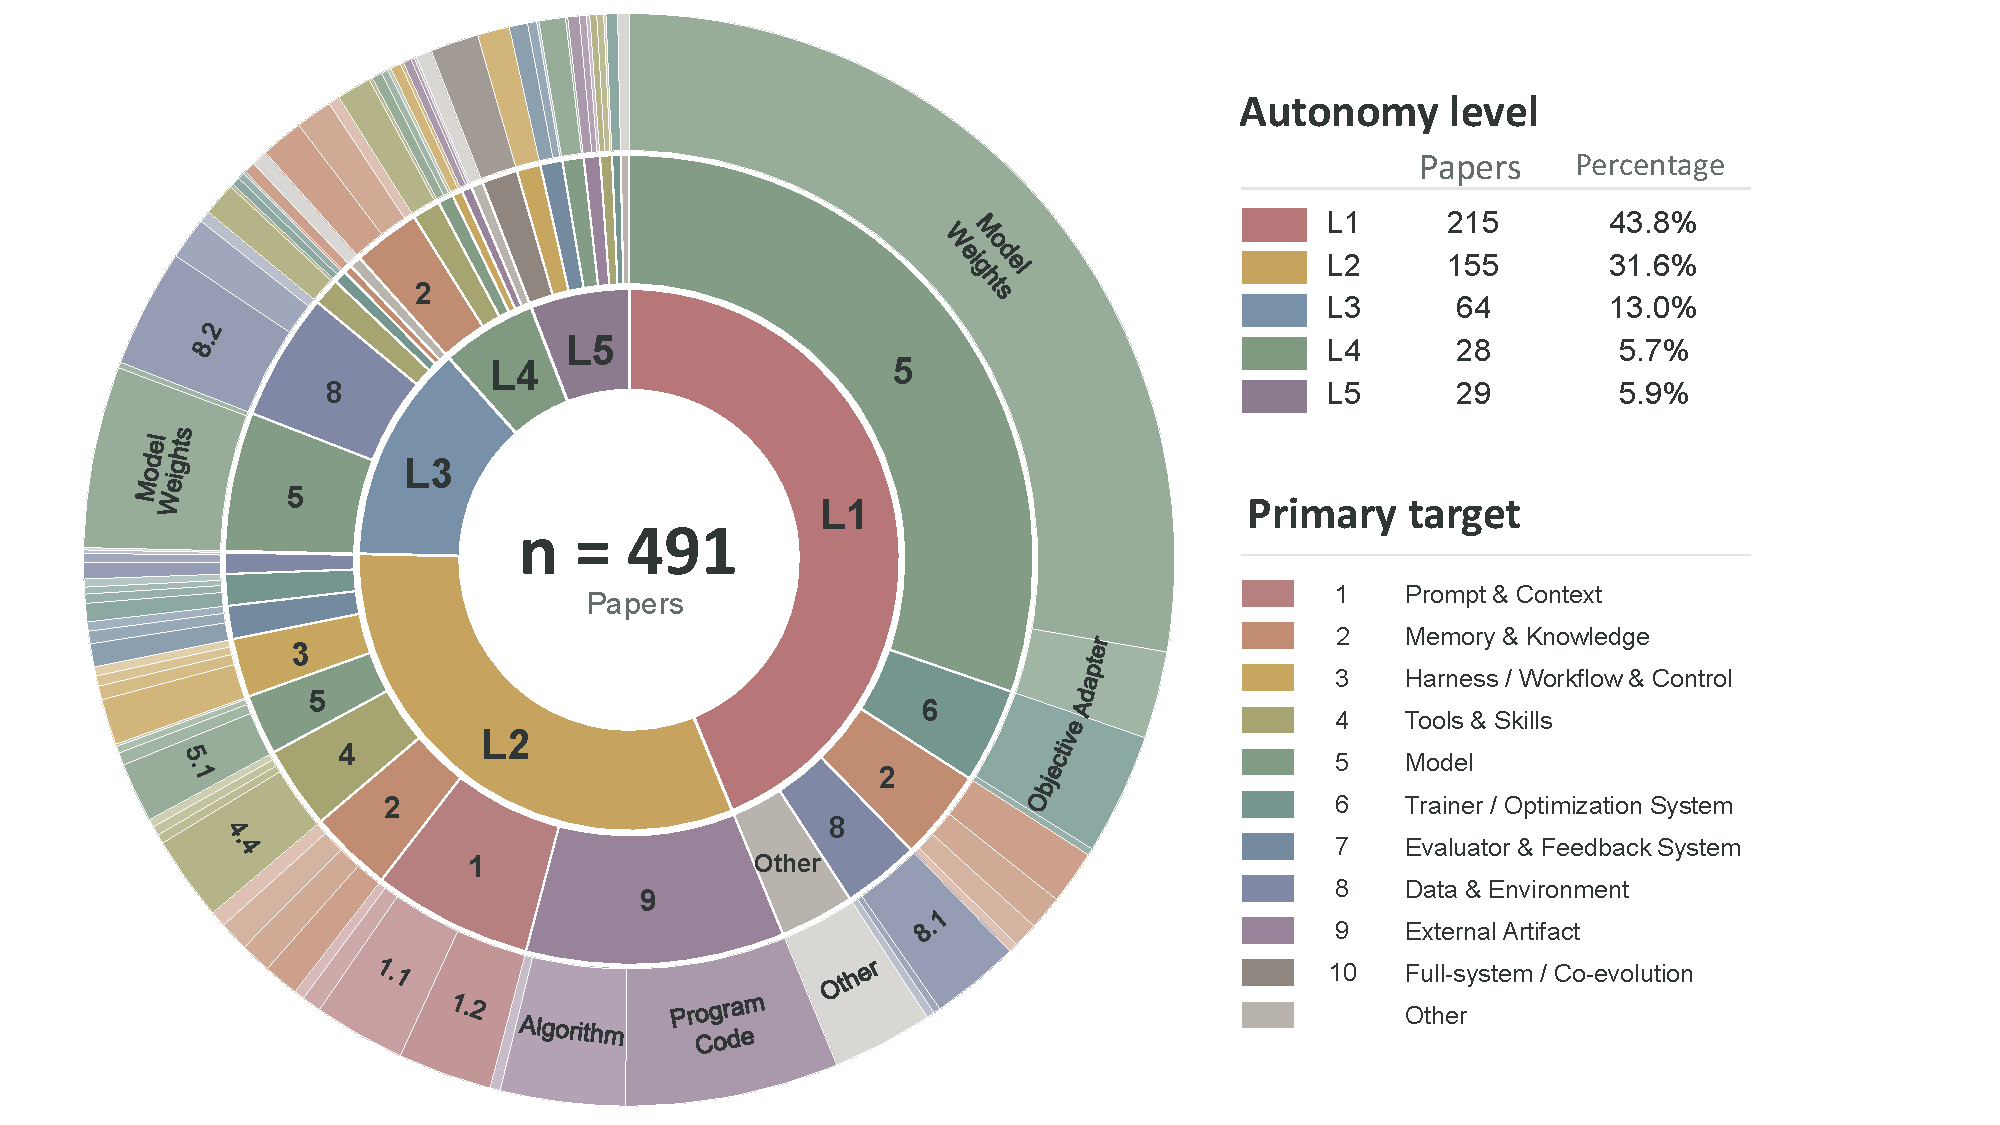
\includegraphics[
        width=\linewidth,
        height=0.72\textheight,
        keepaspectratio
    ]{figures/RSI-Landscape.pdf}
    \caption{
        \textbf{RSI Landscape: Autonomy Levels and Improvement Targets.}
        Distribution of 491 surveyed papers.
        The inner, middle, and outer rings represent autonomy
        levels (L1--L5), primary improvement targets, and
        sub-targets, respectively.
        Autonomy-level percentages are based on paper counts.
        Papers associated with multiple improvement targets
        contribute fractional weights to the target categories.
    }
    \label{fig:rsi-landscape}
\end{figure}

% \clearpage

% ==================================================
% Taxonomy of RSI Improvement Targets
% ==================================================

Table~\ref{tab:rsi-target-taxonomy} details the primary targets and sub-targets represented in Figure~\ref{fig:rsi-landscape}.

\captionsetup[longtable]{
    justification=centering,
    singlelinecheck=false
}
\begingroup
\small   
\renewcommand{\arraystretch}{1.08}
\setlength{\tabcolsep}{4pt}

% The outer table has three visual columns. Each target group is one physical
% longtable row; columns 2--3 are rendered as a nested two-column table.
% This makes the Primary Target cell exactly vertically centered over the
% full height of all sub-target rows, without manual multirow offsets.
\begin{longtable}{
    >{\RaggedRight\arraybackslash}m{0.18\linewidth}
    >{\RaggedRight\arraybackslash}m{0.27\linewidth}
    >{\RaggedRight\arraybackslash}m{0.49\linewidth}
}

\caption{
\textbf{Taxonomy of Improvement Targets in Recursive Self-Improvement Systems.}
The taxonomy decomposes the improvement targets represented in Fig.~\ref{fig:rsi-landscape} into primary targets and sub-targets.
For each sub-target, the table specifies the concrete system component subject to modification.
}
\label{tab:rsi-target-taxonomy}\\

\toprule
\textbf{Primary Target}
& \textbf{Sub-target}
& \textbf{Modified Component}
\\
\midrule
\endfirsthead

\multicolumn{3}{c}{\textit{Table~\ref{tab:rsi-target-taxonomy} continued}}\\
\toprule
\textbf{Primary Target}
& \textbf{Sub-target}
& \textbf{Modified Component}
\\
\midrule
\endhead

\midrule
\multicolumn{3}{r}{\textit{Continued on next page}}\\
\endfoot

\bottomrule
\endlastfoot

% 1. Prompt & Context
1. Prompt \& Context
& \multicolumn{2}{@{}l@{}}{%
\begin{tabular}{
    >{\RaggedRight\arraybackslash}m{0.27\linewidth}
    >{\RaggedRight\arraybackslash}m{0.49\linewidth}
}
1.1 Instruction
& System prompts, role specifications, behavioral rules, constraints, and high-level instructions \\
\subsep
1.2 Task Prompt / Template
& Task descriptions, problem formulations, prompt templates, and reusable task specifications \\
\subsep
1.3 Reasoning Prompt / Protocol
& Explicit reasoning instructions and protocols, including chain-of-thought, reflection, critique, and debate \\
\subsep
1.4 Demonstrations / Exemplars
& Few-shot examples, demonstrations, successful trajectories, and worked solutions included in context \\
\subsep
1.5 Context Composition
& Context selection, ordering, compression, summarization, and allocation of the available context budget \\
\end{tabular}%
}\\
\midrule

% 2. Memory & Knowledge
2. Memory \& Knowledge
& \multicolumn{2}{@{}l@{}}{%
\begin{tabular}{
    >{\RaggedRight\arraybackslash}m{0.27\linewidth}
    >{\RaggedRight\arraybackslash}m{0.49\linewidth}
}
2.1 Episodic / Experience Memory
& Records of prior interactions, execution trajectories, successful and failed attempts, and task-specific reflections \\
\subsep
2.2 Semantic / Knowledge Memory
& Persistent factual, conceptual, and domain knowledge, including structured or external knowledge stores \\
\subsep
2.3 Procedural Memory
& Reusable strategies, experience-derived rules, heuristics, procedures, and playbooks \\
\subsep
2.4 Memory Representation / Organization
& Memory schemas, hierarchical structures, summaries, graphs, indexes, and vector representations \\
\subsep
2.5 Memory Operations
& Policies governing memory writing, retrieval, updating, consolidation, prioritization, and forgetting \\
\end{tabular}%
}\\
\midrule

% 3. Harness / Workflow & Control
3. Harness / Workflow \& Control
& \multicolumn{2}{@{}l@{}}{%
\begin{tabular}{
    >{\RaggedRight\arraybackslash}m{0.27\linewidth}
    >{\RaggedRight\arraybackslash}m{0.49\linewidth}
}
3.1 Workflow / Graph
& Agent graphs, pipelines, nodes, edges, and execution dependencies between computational stages \\
\subsep
3.2 Planning / Decomposition
& Task decomposition, planning modules, subgoal structures, and execution order \\
\subsep
3.3 Routing / Scheduling
& Model routing, agent routing, tool routing, execution scheduling, and computational resource allocation \\
\subsep
3.4 Verification / Reflection Loop
& Control loops for checking and revising intermediate or final outputs, including critic--revise, verify--retry, and reflection procedures \\
\subsep
3.5 Multi-agent Structure / Protocol
& Agent population, role assignment, interaction topology, coordination mechanisms, and communication protocols \\
\subsep
3.6 Harness Implementation / Scaffold Code
& Source code implementing the agent scaffold, orchestration logic, workflow controller, and runtime coordination mechanisms \\
\end{tabular}%
}\\
\midrule

% 4. Tools & Skills
4. Tools \& Skills
& \multicolumn{2}{@{}l@{}}{%
\begin{tabular}{
    >{\RaggedRight\arraybackslash}m{0.27\linewidth}
    >{\RaggedRight\arraybackslash}m{0.49\linewidth}
}
4.1 Tool Set / Inventory
& The collection of tools, APIs, external services, and callable capabilities available to the system \\
\subsep
4.2 Tool Definition / Interface
& Tool descriptions, function signatures, schemas, API wrappers, and input--output specifications \\
\subsep
4.3 Tool Implementation
& Executable code and internal logic implementing tools or callable external functions \\
\subsep
4.4 Skill / Macro Library
& Reusable skills, macros, subroutines, procedures, and higher-level behavioral modules \\
\subsep
4.5 Skill Composition
& Rules and structures for combining lower-level skills into higher-level procedures or capabilities \\
\end{tabular}%
}\\
\midrule

% 5. Model
5. Model
& \multicolumn{2}{@{}l@{}}{%
\begin{tabular}{
    >{\RaggedRight\arraybackslash}m{0.27\linewidth}
    >{\RaggedRight\arraybackslash}m{0.49\linewidth}
}
5.1 Model Weights
& Trainable parameters of the backbone model \\
\subsep
5.2 Adapter / Auxiliary Module
& Parameters of LoRA modules, adapters, memory modules, and other trainable auxiliary components \\
\subsep
5.3 Architecture
& Network architecture, module composition, connectivity patterns, and computational structure \\
\subsep
5.4 Inference Policy / Configuration
& Persistent decoding strategies, test-time policies, inference configurations, and runtime model settings \\
\end{tabular}%
}\\
\midrule

% 6. Trainer / Optimization System
6. Trainer / Optimization System
& \multicolumn{2}{@{}l@{}}{%
\begin{tabular}{
    >{\RaggedRight\arraybackslash}m{0.27\linewidth}
    >{\RaggedRight\arraybackslash}m{0.49\linewidth}
}
6.1 Training Objective
& Loss functions, training rewards, learning objectives, and optimization criteria \\
\subsep
6.2 Optimizer / Update Rule
& Optimizers, parameter-update algorithms, learning-rate policies, and associated hyperparameters \\
\subsep
6.3 Training Schedule / Pipeline
& Ordering, configuration, and interaction of training stages such as fine-tuning, reinforcement learning, and distillation \\
\subsep
6.4 Data Selection / Curriculum
& Training-sample selection rules, data mixtures, difficulty schedules, and curriculum policies \\
\subsep
6.5 Search / Meta-optimization Procedure
& Evolutionary, search, selection, and meta-optimization procedures used to generate and select candidate improvements \\
\end{tabular}%
}\\
\midrule

% 7. Evaluator & Feedback System
7. Evaluator \& Feedback System
& \multicolumn{2}{@{}l@{}}{%
\begin{tabular}{
    >{\RaggedRight\arraybackslash}m{0.27\linewidth}
    >{\RaggedRight\arraybackslash}m{0.49\linewidth}
}
7.1 Evaluator / Judge
& Evaluators, critics, graders, judge models, and related components for assessing candidate outputs or system variants \\
\subsep
7.2 Reward / Fitness Function
& Reward models, fitness functions, utility functions, preference models, and scoring rules \\
\subsep
7.3 Verifier
& Correctness verifiers, test generators, proof checkers, consistency checks, and validation mechanisms \\
\subsep
7.4 Feedback / Credit Assignment
& Mechanisms that transform observed outcomes into localized, aggregated, or temporally assigned improvement signals \\
\end{tabular}%
}\\
\midrule

% 8. Data & Environment
8. Data \& Environment
& \multicolumn{2}{@{}l@{}}{%
\begin{tabular}{
    >{\RaggedRight\arraybackslash}m{0.27\linewidth}
    >{\RaggedRight\arraybackslash}m{0.49\linewidth}
}
8.1 Training / Experience Data
& Training datasets, replay buffers, experience pools, interaction trajectories, and other data used for subsequent learning \\
\subsep
8.2 Task / Curriculum Generator
& Components that generate tasks, problems, challenges, or training episodes for subsequent improvement cycles \\
\subsep
8.3 Environment / Simulator
& Environment dynamics, simulators, interaction rules, task worlds, and structures governing system--environment interaction \\
\subsep
8.4 World Model
& Learned models used to represent, predict, generate, or simulate environmental states and dynamics \\
\end{tabular}%
}\\
\midrule

% 9. External Artifact
9. External Artifact
& \multicolumn{2}{@{}l@{}}{%
\begin{tabular}{
    >{\RaggedRight\arraybackslash}m{0.27\linewidth}
    >{\RaggedRight\arraybackslash}m{0.49\linewidth}
}
9.1 Program / Solution Code
& Task-level programs, patches, or solution code produced by the system, excluding code implementing the agent itself \\
\subsep
9.2 Algorithm
& Algorithms, kernels, mathematical procedures, symbolic methods, and computational techniques \\
\subsep
9.3 Scientific / Design Artifact
& Scientific hypotheses, experimental designs, architectures, circuits, engineering designs, and related research artifacts \\
\end{tabular}%
}\\
\midrule

% 10. Full-system / Co-evolution
10. Full-system / Co-evolution
& \multicolumn{2}{@{}l@{}}{%
\begin{tabular}{
    >{\RaggedRight\arraybackslash}m{0.27\linewidth}
    >{\RaggedRight\arraybackslash}m{0.49\linewidth}
}
10.1 Multi-target Harness
& Multiple harness-level components jointly modified within the same improvement process, such as prompts, memory, workflows, and tools \\
\subsep
10.2 Model--Harness Co-evolution
& Model parameters and surrounding harness or scaffold components jointly modified across improvement cycles \\
\subsep
10.3 Improvement-loop / Meta-RSI
& The mechanism that generates, evaluates, selects, and applies candidate changes across successive improvement cycles \\
\end{tabular}%
}\\

\end{longtable}
\endgroup



% ==================================================
% Appendix B: Industry Landscape
% ==================================================


% \appsection{Industry Landscape}
% \label{app:industry-landscape}

% \begin{landscape}
% \pagestyle{appendixBstyle}
% \newcolumntype{P}[1]{>{\RaggedRight\arraybackslash\hspace{0pt}}p{#1}}
\newcolumntype{I}[1]{>{\Centering\arraybackslash\hspace{0pt}}p{#1}}
\newcommand{\src}[1]{\href{#1}{\textcolor{blue!55!black}{\faGlobe}}}
\newcommand{\sectionrow}[2]{%
  \multicolumn{7}{@{}p{\dimexpr\linewidth-2\tabcolsep\relax}@{}}{%
    \cellcolor{black!7}\strut\textbf{#1}\hspace{0.8em}\textcolor{black!65}{\scriptsize #2}}\\[-0.1ex]
}
\newcommand{\innerline}{\arrayrulecolor{black!13}\cline{2-7}\arrayrulecolor{black}}
\setlength{\emergencystretch}{2em}
\urlstyle{same}
\raggedbottom
\pagestyle{plain}
\begin{center}
{\large\bfseries Company Archetypes in the Emerging RSI / Self-Improvement Landscape}\\[2pt]
{\footnotesize One row per product or representative work; 72 distinct companies/teams; public-source snapshot: September 2026}
\end{center}
\vspace{-0.35em}
\noindent
{\scriptsize\textit{Organization principle: company archetype, not geography. The RSI tag is a compact mapping to the B0--L5 scheme and is not a claim that the company itself uses that label. \faGlobe\ = clickable primary source.}}
\vspace{0.35em}
\begingroup
\fontsize{7.15}{8.20}\selectfont
\setlength{\tabcolsep}{2.0pt}
\renewcommand{\arraystretch}{1.02}
\begin{longtable}{
  P{2.72cm}
  P{4.69cm}
  P{3.10cm}
  P{4.15cm}
  P{4.45cm}
  P{2.06cm}
  I{0.78cm}}
\caption{RSI / self-improvement company landscape organized by company archetype.}\label{tab:industry-landscape}\\
\toprule
\textbf{Company} &
\textbf{Product / representative work} &
\textbf{Sub-scenario} &
\textbf{Improvement target / artifact} &
\textbf{AI-controlled part} &
\textbf{RSI relation} &
\textcolor{blue!55!black}{\faGlobe} \\
\midrule
\endfirsthead
\multicolumn{7}{c}{\tablename\ \thetable\ -- continued}\\
\toprule
\textbf{Company} &
\textbf{Product / representative work} &
\textbf{Sub-scenario} &
\textbf{Improvement target / artifact} &
\textbf{AI-controlled part} &
\textbf{RSI relation} &
\textcolor{blue!55!black}{\faGlobe} \\
\midrule
\endhead
\midrule
\multicolumn{7}{r}{\footnotesize continued on next page}\\
\endfoot
\bottomrule
\endlastfoot
\sectionrow{A. Frontier foundation-model \& general-agent labs}{Broad model/platform labs; RSI appears as one capability frontier rather than the sole company thesis.}
\multirow[t]{7}{2.72cm}{\RaggedRight\textbf{OpenAI}} & Research acceleration / automated research intern & AI-for-AI research & research code; experiments; evals & code; experiments; candidate integration & L2 & \src{https://openai.com/index/research-acceleration-view-inside-openai/} \\*
\innerline
 & GPT-Red & self-play robustness & red-team policy; adversarial data & attack; defend; train; evaluate & L2 & \src{https://openai.com/index/unlocking-self-improvement-gpt-red/} \\*
\innerline
 & Self-improving tax agents & production adaptation & agent code; prompts; eval set & mine failures; patch; evaluate & L4 cand. & \src{https://openai.com/index/building-self-improving-tax-agents-with-codex/} \\*
\innerline
 & Harness Engineering & agent-first software R\&D & repo; CI; agent instructions & code; test; PR; repair & L1-L2 adj. & \src{https://openai.com/index/harness-engineering/} \\*
\innerline
 & Symphony & agent orchestration & task state; repo; workflows & schedule; execute; handoff & L1 adj. & \src{https://github.com/openai/symphony} \\*
\innerline
 & AgentKit / prompt optimizer / RFT & agent optimization stack & prompts; graders; weights & optimize; grade; fine-tune & L1-L2 & \src{https://openai.com/index/introducing-agentkit/} \\*
\innerline
 & Deep Research & autonomous research & task-local evidence & search; browse; synthesize & B0 & \src{https://openai.com/index/introducing-deep-research/} \\
\addlinespace[0.85pt]
\multirow[t]{9}{2.72cm}{\RaggedRight\textbf{Anthropic}} & When AI builds itself & RSI roadmap & AI-development process & code; experiments; future successor design & L5 target & \src{https://www.anthropic.com/institute/recursive-self-improvement} \\*
\innerline
 & Automated Weak-to-Strong Researcher & automated alignment research & hypotheses; code; experiment logs & propose; train; evaluate; share & L2 & \src{https://alignment.anthropic.com/2026/automated-w2s-researcher/} \\*
\innerline
 & Tool optimization with Claude & tool self-optimization & tool specs; implementations & analyze traces; rewrite; evaluate & L2 & \src{https://www.anthropic.com/engineering/writing-tools-for-agents} \\*
\innerline
 & Harness design for long-running apps & autonomous software R\&D & harness; evaluator; app code & plan; generate; evaluate; iterate & L2 adj. & \src{https://www.anthropic.com/engineering/harness-design-long-running-apps} \\*
\innerline
 & Effective long-running agent harnesses & cross-context persistence & progress files; git state & initialize; code; handoff & L1 adj. & \src{https://www.anthropic.com/engineering/effective-harnesses-for-long-running-agents} \\*
\innerline
 & Agent Skills & persistent skill substrate & skills; scripts; resources & discover; load; reuse & L1 enabler & \src{https://www.anthropic.com/engineering/equipping-agents-for-the-real-world-with-agent-skills} \\*
\innerline
 & Multi-agent Research & autonomous research & task-local findings & plan; spawn; search; synthesize & B0 & \src{https://www.anthropic.com/engineering/multi-agent-research-system} \\*
\innerline
 & Managed Agents & long-horizon agent infrastructure & stable interface; harness & run; resume; supervise & L1 enabler & \src{https://www.anthropic.com/engineering/managed-agents} \\*
\innerline
 & Parallel Claude compiler project & autonomous software engineering & shared codebase; tests & decompose; code; test; coordinate & B0-L1 adj. & \src{https://www.anthropic.com/engineering/building-c-compiler} \\
\addlinespace[0.85pt]
\multirow[t]{3}{2.72cm}{\RaggedRight\textbf{Google DeepMind}} & AlphaEvolve & task-specific program search & algorithms; kernels; system code & generate; mutate; evaluate; select & B0 & \src{https://deepmind.google/blog/alphaevolve-a-gemini-powered-coding-agent-for-designing-advanced-algorithms/} \\*
\innerline
 & AI Co-Scientist & scientific hypothesis search & hypotheses; research proposals & generate; debate; rank; refine & L2 adj. & \src{https://research.google/blog/accelerating-scientific-breakthroughs-with-an-ai-co-scientist/} \\*
\innerline
 & AlphaChip & AI-for-hardware co-design & chip layouts; design policy & place; score; learn; transfer & L2 adj. & \src{https://deepmind.google/blog/how-alphachip-transformed-computer-chip-design/} \\
\addlinespace[0.85pt]
\multirow[t]{2}{2.72cm}{\RaggedRight\textbf{NVIDIA}} & Eureka & reward / policy design & reward code; robot policies & reward synthesis; simulation; policy training & L2 & \src{https://arxiv.org/abs/2310.12931} \\*
\innerline
 & ASPIRE & reward / policy design & reward code; robot policies & reward synthesis; simulation; policy training & L2 & \src{https://research.nvidia.com/labs/gear/aspire/} \\
\addlinespace[0.85pt]
\multirow[t]{5}{2.72cm}{\RaggedRight\textbf{Microsoft}} & Agent Lightning & agent reinforcement learning & policy weights; experience traces & collect; credit; train; evaluate & L2 & \src{https://www.microsoft.com/en-us/research/project/agent-lightning/} \\*
\innerline
 & Agent Lightning v1.0 & harnessed agentic RL & harness traces; policy weights & interact; retokenize; train; benchmark & L2 & \src{https://www.microsoft.com/en-us/research/publication/agent-lightning-v1-0-towards-harnessed-agentic-rl/} \\*
\innerline
 & SkillOpt & skill optimization & skill files; instructions & edit; evaluate; optimize & L2 & \src{https://www.microsoft.com/en-us/research/blog/skillopt-agent-skills-as-trainable-parameters/} \\*
\innerline
 & ReVeal & self-verifying code agents & code; tests; verifier policy & generate; verify; revise; scale & L2 & \src{https://www.microsoft.com/en-us/research/publication/reveal-self-evolving-code-agents-via-reliable-self-verification/} \\*
\innerline
 & Universal Verifier / auto-research & agent verification R\&D & rubrics; verifier; eval pipeline & design; test; compare; refine & L2 adj. & \src{https://www.microsoft.com/en-us/research/articles/the-art-of-building-verifiers-for-computer-use-agents/} \\
\addlinespace[0.85pt]
\multirow[t]{2}{2.72cm}{\RaggedRight\textbf{Meta}} & Self-Taught Evaluator & evaluator self-training & judge model; synthetic preferences & generate; judge; train; iterate & L2 & \src{https://ai.meta.com/blog/fair-news-segment-anything-2-1-meta-spirit-lm-layer-skip-salsa-lingua/} \\*
\innerline
 & HyperAgents & meta-agent self-modification & task agent; meta agent; program & solve; self-edit; evaluate; archive & L5 cand. & \src{https://ai.meta.com/research/publications/hyperagents/} \\
\addlinespace[0.85pt]
\multirow[t]{3}{2.72cm}{\RaggedRight\textbf{Alibaba / Qwen}} & Qwen-Agent & agent training / synthetic environments & training data; environments; post-training & simulation; data synthesis; tool use; RL & L1-L2 & \src{https://qwenlm.github.io/blog/qwen-agent-2405/} \\*
\innerline
 & AgentWorld & agent training / synthetic environments & training data; environments; post-training & simulation; data synthesis; tool use; RL & L1-L2 & \src{https://qwen.ai/blog?id=qwen-agentworld} \\*
\innerline
 & Qwen-Scope & agent training / synthetic environments & training data; environments; post-training & simulation; data synthesis; tool use; RL & L1-L2 & \src{https://arxiv.org/abs/2605.11887} \\
\addlinespace[0.85pt]
\multirow[t]{2}{2.72cm}{\RaggedRight\textbf{DeepSeek}} & R1 & reasoning self-bootstrapping & reasoning policy; verifier & self-generated reasoning; RL; verifier iteration & L2 & \src{https://github.com/deepseek-ai/DeepSeek-R1} \\*
\innerline
 & Math-V2 & reasoning self-bootstrapping & reasoning policy; verifier & self-generated reasoning; RL; verifier iteration & L2 & \src{https://github.com/deepseek-ai/DeepSeek-Math-V2} \\
\addlinespace[0.85pt]
\RaggedRight\textbf{Tencent AI Lab} & R-Zero & self-play reasoning & tasks; pseudo-labels; policy weights & challenge generation; solve; vote; RL & L2-L3 & \src{https://arxiv.org/abs/2508.05004} \\
\addlinespace[0.85pt]
\multirow[t]{2}{2.72cm}{\RaggedRight\textbf{ByteDance Seed}} & Seed-Thinking & model / agent post-training & data; reward; policy weights & data filtering; reward verification; RL & L1-L2 & \src{https://github.com/ByteDance-Seed} \\*
\innerline
 & Seed1.5-VL & model / agent post-training & data; reward; policy weights & data filtering; reward verification; RL & L1-L2 & \src{https://seed.bytedance.com/zh/blog/bytedance-s-latest-thinking-model-seed-thinking-v1-5-technical-details-disclosed} \\
\addlinespace[0.85pt]
\multirow[t]{3}{2.72cm}{\RaggedRight\textbf{MiniMax}} & M2 & persistent cloud agents & memory; skills; agent policy & tool use; long-run execution; skill reuse & L1-L2 & \src{https://www.minimax.io/news/minimax-m2} \\*
\innerline
 & MaxHermes & persistent cloud agents & memory; skills; agent policy & tool use; long-run execution; skill reuse & L1-L2 & \src{https://www.maxhermes.dev/en} \\*
\innerline
 & MaxClaw & persistent cloud agents & memory; skills; agent policy & tool use; long-run execution; skill reuse & L1-L2 & \src{https://agent.minimaxi.com/activity/max-claw} \\
\addlinespace[0.85pt]
\multirow[t]{2}{2.72cm}{\RaggedRight\textbf{Moonshot AI}} & Kimi K3 & long-horizon agents & agent orchestration; tool policy & planning; tool use; swarm coordination & L1-L2 adj. & \src{https://www.moonshot.cn/} \\*
\innerline
 & Agent Swarm & long-horizon agents & agent orchestration; tool policy & planning; tool use; swarm coordination & L1-L2 adj. & \src{https://www.moonshot.cn/} \\
\addlinespace[0.85pt]
\multirow[t]{2}{2.72cm}{\RaggedRight\textbf{Zhipu AI / Z.AI}} & AutoGLM & computer-use agent training & policy weights; virtual-phone environments & perception; planning; action; RL & L2 & \src{https://autoglm.z.ai/blog/} \\*
\innerline
 & AgentRL & computer-use agent training & policy weights; virtual-phone environments & perception; planning; action; RL & L2 & \src{https://docs.z.ai/guides/vlm/autoglm-phone-multilingual} \\
\addlinespace[0.85pt]
\multirow[t]{2}{2.72cm}{\RaggedRight\textbf{Deep Cogito}} & Cogito v2 & reasoning post-training & reasoning policy; weights & search; distill; iterative alignment & L1-L2 & \src{https://www.deepcogito.com/research/cogito-v2-preview} \\*
\innerline
 & IDA & reasoning post-training & reasoning policy; weights & search; distill; iterative alignment & L1-L2 & \src{https://www.deepcogito.com/research/cogito-v2-1} \\
\addlinespace[0.85pt]
\RaggedRight\textbf{Poolside} & Model Factory & automated model R\&D & synthetic data; RL; architecture & eval; code-exec RL; ablations; data mix & L1-L2 & \src{https://poolside.ai/research} \\
\addlinespace[0.85pt]
\multirow[t]{2}{2.72cm}{\RaggedRight\textbf{Thinking Machines Lab}} & Tinker Agent RL & model customization / agent RL & policy weights; tool-use policy & RL; LLM-judge grading; tool discovery & L1-L2 & \src{https://tinker-docs.thinkingmachines.ai/cookbook/recipes/agent-rl/} \\*
\innerline
 & Inkling & model customization / agent RL & policy weights; tool-use policy & RL; LLM-judge grading; tool discovery & L1-L2 & \src{https://thinkingmachines.ai/news/introducing-inkling/} \\
\addlinespace[0.85pt]
\multirow[t]{2}{2.72cm}{\RaggedRight\textbf{Nous Research}} & Hermes Agent & persistent agents & skills; memory; tool gateway & memory; skill reuse; tool orchestration & L1-L2 & \src{https://github.com/NousResearch/hermes-agent} \\*
\innerline
 & skills / memory & persistent agents & skills; memory; tool gateway & memory; skill reuse; tool orchestration & L1-L2 & \src{https://hermes-agent.nousresearch.com/docs} \\
\addlinespace[0.85pt]
\sectionrow{B. RSI-native / AI4AI companies}{Self-improvement, AI-for-AI, self-evolution, or recursive improvement is central to the company/research thesis.}
\RaggedRight\textbf{Ricursive Intelligence} & AI-chip co-design & AI systems / chips & EDA designs; compute stack & design search; verify; iterate & L2; L5 vision & \src{https://www.ricursive.com/} \\
\addlinespace[0.85pt]
\RaggedRight\textbf{Recursive} & Automated AI Research & model-training research & training recipes; kernels; code & ideas; experiments; branch merge & L2 & \src{https://www.recursive.com/articles/first-steps-toward-automated-ai-research} \\
\addlinespace[0.85pt]
\multirow[t]{2}{2.72cm}{\RaggedRight\textbf{Imbue}} & Catalyst & research search & recipes; code; hypotheses & population search; experiments; interpretation & L2-L3 & \src{https://github.com/imbue-ai/catalyst} \\*
\innerline
 & Darwinian Evolver & research search & recipes; code; hypotheses & population search; experiments; interpretation & L2-L3 & \src{https://imbue.com/blog/2026-07-20-imbue-catalyst-nanochat} \\
\addlinespace[0.85pt]
\RaggedRight\textbf{Weco AI} & AIDE2 & meta-improvement of researcher & research harness; improver code & rewrite improver; eval; inheritance & L5 cand. & \src{https://www.weco.ai/blog/first-evidence-of-recursive-self-improvement} \\
\addlinespace[0.85pt]
\multirow[t]{2}{2.72cm}{\RaggedRight\textbf{Sakana AI}} & Darwin Godel Machine & self-editing agents / AI research & agent source; research pipeline & self-modify; benchmark; archive; experiments & L5 cand. & \src{https://arxiv.org/abs/2505.22954} \\*
\innerline
 & AI Scientist & self-editing agents / AI research & agent source; research pipeline & self-modify; benchmark; archive; experiments & L5 cand. & \src{https://github.com/SakanaAI/AI-Scientist} \\
\addlinespace[0.85pt]
\multirow[t]{3}{2.72cm}{\RaggedRight\textbf{Evolvent AI}} & Org self-evolving agents & software-agent evolution & skills; memory; code; environments & tasks; feedback; refactor; skill updates & L2-L3 & \src{https://evolvent.co/zh/blog/org-self-evolving-agents} \\*
\innerline
 & RSIBench & software-agent evolution & skills; memory; code; environments & tasks; feedback; refactor; skill updates & L2-L3 & \src{https://evolvent.co/zh/blog/RSIBench-Data} \\*
\innerline
 & Terrarium & software-agent evolution & skills; memory; code; environments & tasks; feedback; refactor; skill updates & L2-L3 & \src{https://evolvent.co/en/blog/terrarium} \\
\addlinespace[0.85pt]
\multirow[t]{2}{2.72cm}{\RaggedRight\textbf{MetaCircle}} & ComfyResearch & AI4AI / autoresearch & training workflows; research hypotheses & experiment compose; code; hypothesis; scoring & L2; L5 vision & \src{https://meta-circle.com/blog/comfyresearch-see-how-learning-happens} \\*
\innerline
 & OPHIS & AI4AI / autoresearch & training workflows; research hypotheses & experiment compose; code; hypothesis; scoring & L2; L5 vision & \src{https://meta-circle.com/blog/ophis-a-new-paradigm-for-autoresearch} \\
\addlinespace[0.85pt]
\multirow[t]{2}{2.72cm}{\RaggedRight\textbf{Frontis AI / Xianyuan}} & OpenRSI & AI4AI / self-improving agents & skills; memory; harness; weights & experience; update search; eval; post-training & L2-L3 & \src{https://github.com/FrontisAI/OpenRSI} \\*
\innerline
 & Frontis-MA1 & AI4AI / self-improving agents & skills; memory; harness; weights & experience; update search; eval; post-training & L2-L3 & \src{https://arxiv.org/abs/2607.28568} \\
\addlinespace[0.85pt]
\multirow[t]{3}{2.72cm}{\RaggedRight\textbf{EvoMap}} & Evolver & shared code evolution & genes / capsules; code assets & generate; test; publish; reuse; adapt & L2-L3 & \src{https://github.com/EvoMap/evolver} \\*
\innerline
 & GEP & shared code evolution & genes / capsules; code assets & generate; test; publish; reuse; adapt & L2-L3 & \src{https://evomap.ai/wiki/16-gep-protocol} \\*
\innerline
 & GeneBench & shared code evolution & genes / capsules; code assets & generate; test; publish; reuse; adapt & L2-L3 & \src{https://evomap.ai/wiki/36-gene-bench-report} \\
\addlinespace[0.85pt]
\RaggedRight\textbf{Endless Frontier} & BigBang-v1 & AI-research data generation & synthetic programs; training data; critic & generate; execute; critique; meta-critique & L2-L3 & \src{https://github.com/endless-frontier/BigBang-v1} \\
\addlinespace[0.85pt]
\multirow[t]{2}{2.72cm}{\RaggedRight\textbf{Mirendil}} & Self-accelerating AI & AI R\&D automation & model code; experiments; research stack & experiment generation; execution; iteration & L2 & \src{https://mirendil.com/news/scaling-self-accelerating-ai-with-google/} \\*
\innerline
 & AI Scientist & AI R\&D automation & model code; experiments; research stack & experiment generation; execution; iteration & L2 & \src{https://www.devvrit.com/} \\
\addlinespace[0.85pt]
\multirow[t]{3}{2.72cm}{\RaggedRight\textbf{Chaoyan Intelligence*}} & TUMIX & self-evolving research models & research policy; tool-use policy & questioning; experiments; code; self-check & L2-L3 & \src{https://arxiv.org/abs/2510.01279} \\*
\innerline
 & R1-Code-Interpreter & self-evolving research models & research policy; tool-use policy & questioning; experiments; code; self-check & L2-L3 & \src{https://arxiv.org/abs/2505.21668} \\*
\innerline
 & AI Scientist & self-evolving research models & research policy; tool-use policy & questioning; experiments; code; self-check & L2-L3 & \src{https://www.qbitai.com/2026/07/455041.html} \\
\addlinespace[0.85pt]
\multirow[t]{2}{2.72cm}{\RaggedRight\textbf{Theseus}} & Argus & long-horizon self-evolving agents & experience; memory; environment setup & plan; code; review; experience writeback & L2-L3 & \src{https://arxiv.org/abs/2608.05144} \\*
\innerline
 & SetupX & long-horizon self-evolving agents & experience; memory; environment setup & plan; code; review; experience writeback & L3 & \src{https://arxiv.org/abs/2605.26186} \\
\addlinespace[0.85pt]
\multirow[t]{2}{2.72cm}{\RaggedRight\textbf{Adaption Labs}} & AutoScientist & AI-research automation & training recipes; datasets; code & research plan; experiments; selection & L2 & \src{https://docs.adaptionlabs.ai/autoscientist/overview/} \\*
\innerline
 & Forge & AI-research automation & training recipes; datasets; code & research plan; experiments; selection & L2 & \src{https://docs.adaptionlabs.ai/api/resources/autoscientist} \\
\addlinespace[0.85pt]
\sectionrow{C. Autonomous R\&D \& scientific-discovery companies}{Primary product is automated research/discovery; RSI relevance comes from automating experiment and knowledge-production loops.}
\RaggedRight\textbf{Periodic Labs} & Autonomous laboratory & AI for science & hypotheses; experiment data; models & experiment design; lab run; learning & L3 cand. & \src{https://periodic.com/} \\
\addlinespace[0.85pt]
\RaggedRight\textbf{FutureHouse} & BixBench & AI-scientist evaluation & research tasks; benchmark frontier & bioinformatics workflows; open-ended eval & B0-L2 adj. & \src{https://github.com/Future-House/BixBench} \\
\addlinespace[0.85pt]
\RaggedRight\textbf{Edison Scientific} & Kosmos & autonomous science & hypotheses; code; scientific artifacts & literature; experiments; synthesis & L2-L3 & \src{https://arxiv.org/abs/2511.02824} \\
\addlinespace[0.85pt]
\multirow[t]{2}{2.72cm}{\RaggedRight\textbf{Axiom Math}} & Putnam 2025 & formal mathematics & proofs; verifier traces & conjecture; proof search; formal verification & L2 & \src{https://github.com/AxiomMath/putnam2025} \\*
\innerline
 & IMO 2026 & formal mathematics & proofs; verifier traces & conjecture; proof search; formal verification & L2 & \src{https://github.com/AxiomMath/IMO2026} \\
\addlinespace[0.85pt]
\RaggedRight\textbf{Harmonic} & Aristotle & theorem proving & formal proofs & translate; prove; verify & L1-L2 & \src{https://harmonic.fun/pdf/Aristotle_IMO_Level_Automated_Theorem_Proving.pdf} \\
\addlinespace[0.85pt]
\RaggedRight\textbf{Core Automation} & AI systems-research stack & automated systems research & systems code; research hypotheses & design; code; benchmark; iterate & L2 cand. & \src{https://www.coreauto.com/blog} \\
\addlinespace[0.85pt]
\RaggedRight\textbf{Discovery Loop} & Autonomous discovery loop & automated experimentation & protocols; findings & hypothesis; experiment; analysis; next-step & L3 cand. & \src{https://www.discoveryloop.com/} \\
\addlinespace[0.85pt]
\RaggedRight\textbf{Lila Sciences} & Autonomous Science platform & scientific discovery & hypotheses; experiments; post-training data & design; lab execution; real-time learning & L3 cand. & \src{https://www.lila.ai/} \\
\addlinespace[0.85pt]
\RaggedRight\textbf{Karpathy / autoresearch} & autoresearch & narrow automated research & training code; configs & edit; train; measure; keep & L2 & \src{https://github.com/karpathy/autoresearch} \\
\addlinespace[0.85pt]
\multirow[t]{2}{2.72cm}{\RaggedRight\textbf{Prime Intellect}} & Autonomous research & model R\&D & training recipe; optimizer; code & hypothesis; GPU runs; ablation & L2 & \src{https://www.primeintellect.ai/blog/measuring-autonomous-research} \\*
\innerline
 & Speedrun Frontier & model R\&D & training recipe; optimizer; code & hypothesis; GPU runs; ablation & L2 & \src{https://github.com/PrimeIntellect-ai/experiments-autonomous-speedrunning} \\
\addlinespace[0.85pt]
\RaggedRight\textbf{Analemma} & FARS & autonomous research & proposals; code; logs; papers & topic; experiment; analysis; writing & L2-L3 & \src{https://fars-live.analemma.ai/blog/introducing-fars/} \\
\addlinespace[0.85pt]
\multirow[t]{3}{2.72cm}{\RaggedRight\textbf{Novix}} & AutoAgent & AI research agent & research workflow; eval harness & idea; tool use; experiments; reporting & L2 & \src{https://github.com/HKUDS/AutoAgent} \\*
\innerline
 & OpenHarness & AI research agent & research workflow; eval harness & idea; tool use; experiments; reporting & L2 & \src{https://github.com/HKUDS/OpenHarness} \\*
\innerline
 & AI-Researcher & AI research agent & research workflow; eval harness & idea; tool use; experiments; reporting & L2 & \src{https://github.com/HKUDS/AI-Researcher} \\
\addlinespace[0.85pt]
\multirow[t]{3}{2.72cm}{\RaggedRight\textbf{UniPat}} & UniScientist & research / evaluation agents & research traces; benchmarks & experiments; coding; multi-agent eval & L1-L2 & \src{https://www.unipat.ai/blog/UniScientist} \\*
\innerline
 & UniSwarm & research / evaluation agents & research traces; benchmarks & experiments; coding; multi-agent eval & L1-L2 & \src{https://www.unipat.ai/blog/UniSwarm} \\*
\innerline
 & UniMath & research / evaluation agents & research traces; benchmarks & experiments; coding; multi-agent eval & L1-L2 & \src{https://www.unipat.ai/blog/UniMath} \\
\addlinespace[0.85pt]
\RaggedRight\textbf{Kai Chen / venture TBD*} & Intern-S1 & AI for science models & scientific model; training data & model training; scientific reasoning & adj.; entity TBD & \src{https://air.tsinghua.edu.cn/info/1008/2492.htm} \\
\addlinespace[0.85pt]
\sectionrow{D. Agent optimization, evaluation \& learning infrastructure}{Infrastructure for feedback, skills, RL, evaluation, simulators, training data, or production-agent improvement.}
\RaggedRight\textbf{Warp} & Skill optimization loop & coding-agent skills & skills; instructions; examples & feedback mining; skill rewrite; eval & L2 & \src{https://www.warp.dev/blog/self-improvement-loop-for-skills} \\
\addlinespace[0.85pt]
\multirow[t]{2}{2.72cm}{\RaggedRight\textbf{Factory}} & Signals & production coding agents & agent behavior; product code & session mining; failure clusters; patch PRs & L4 & \src{https://factory.com/news/factory-signals} \\*
\innerline
 & Software Factory & production coding agents & agent behavior; product code & session mining; failure clusters; patch PRs & L4 & \src{https://factory.ai/news/software-factory} \\
\addlinespace[0.85pt]
\RaggedRight\textbf{LangChain} & LangSmith self-improving evaluators & evaluator alignment & judge prompts; evaluator model & feedback ingest; judge update; eval & L1-L2 & \src{https://docs.langchain.com/langsmith/improve-judge-evaluator-feedback} \\
\addlinespace[0.85pt]
\RaggedRight\textbf{Replit} & Agent 3 & software engineering & application code; tests & build; test; repair; long runs & L1-L2 & \src{https://replit.com/blog/introducing-agent-3-our-most-autonomous-agent-yet} \\
\addlinespace[0.85pt]
\RaggedRight\textbf{MorphMind} & Caliper & agent calibration / org memory & agent skills; shared experience & measure; route; reuse experience & L1-L2 adj. & \src{https://morphmind.ai/products/caliper} \\
\addlinespace[0.85pt]
\multirow[t]{2}{2.72cm}{\RaggedRight\textbf{DatologyAI}} & BeyondWeb & data optimization & training corpus; synthetic data & curate; filter; synthesize; benchmark & L1-L2 & \src{https://www.datologyai.com/blog/beyondweb} \\*
\innerline
 & DatBench & data optimization & training corpus; synthetic data & curate; filter; synthesize; benchmark & L1-L2 & \src{https://www.datologyai.com/blog/datbench-discriminative-faithful-and-efficient-vision-language-model-evaluations} \\
\addlinespace[0.85pt]
\RaggedRight\textbf{Ineffable Intelligence} & RL infrastructure & RL / experience infrastructure & training environments; trajectories & rollouts; reward; distributed RL & L1-L3 enabler & \src{https://www.ineffable.ai/} \\
\addlinespace[0.85pt]
\multirow[t]{2}{2.72cm}{\RaggedRight\textbf{Goodfire}} & Ember & interpretability-driven training & feature activations; reward signals & feature discovery; feedback; RL & L1-L2 & \src{https://www.goodfire.com/research/rlfr} \\*
\innerline
 & RLFR & interpretability-driven training & feature activations; reward signals & feature discovery; feedback; RL & L1-L2 & \src{https://www.goodfire.com/research/rlfr} \\
\addlinespace[0.85pt]
\multirow[t]{2}{2.72cm}{\RaggedRight\textbf{Patronus AI}} & Generative Simulators & evaluation / simulation & simulators; eval suites & scenario generation; grading; failure analysis & L2-L3 enabler & \src{https://www.patronus.ai/blog/introducing-generative-simulators} \\*
\innerline
 & Percival & evaluation / simulation & simulators; eval suites & scenario generation; grading; failure analysis & L2-L3 enabler & \src{https://www.patronus.ai/blog/percival-chat-an-eval-copilot-for-agentic-systems} \\
\addlinespace[0.85pt]
\multirow[t]{2}{2.72cm}{\RaggedRight\textbf{Braintrust}} & Loop & production feedback / eval & prompts; evals; datasets & trace ingest; scoring; prompt optimization & L1-L2 & \src{https://www.braintrust.dev/docs/loop} \\*
\innerline
 & Autoevals & production feedback / eval & prompts; evals; datasets & trace ingest; scoring; prompt optimization & L1-L2 & \src{https://www.braintrust.dev/docs/cookbook/recipes/Loop} \\
\addlinespace[0.85pt]
\multirow[t]{2}{2.72cm}{\RaggedRight\textbf{Mechanize}} & RL environments & experience / eval infrastructure & RL tasks; graders; environments & task design; grading; training signal & L3 enabler & \src{https://www.mechanize.work/} \\*
\innerline
 & GBA Eval & experience / eval infrastructure & RL tasks; graders; environments & task design; grading; training signal & L3 enabler & \src{https://www.mechanize.work/} \\
\addlinespace[0.85pt]
\RaggedRight\textbf{Kando AI} & Early company signal & undisclosed / early-stage & undisclosed & undisclosed & unverified & \src{https://www.preqin.com/data/profile/asset/kando-ai/811935} \\
\addlinespace[0.85pt]
\RaggedRight\textbf{Entropy Order*} & Data-expert platform & high-quality training data & expert data; eval assets & data production; benchmarking & L1-L3 enabler & \src{https://emergeia.com/en/project/2025F-020} \\
\addlinespace[0.85pt]
\RaggedRight\textbf{Compounding Intelligence / CORAL*} & CORAL & multi-agent research & shared notes; skills; logs & parallel experiments; knowledge sharing; eval & L2-L3 & \src{https://human-agent-society.github.io/CORAL} \\
\addlinespace[0.85pt]
\RaggedRight\textbf{Naive.ai*} & Research-lab signal & early RSI lab & undisclosed & undisclosed & RSI claim; unverified & \src{https://naive.ai/} \\
\addlinespace[0.85pt]
\sectionrow{E. Embodied, world-model \& continual-adaptation companies}{Persistent adaptation is tied to world models, robotics, environments, or test-time/continual learning.}
\multirow[t]{2}{2.72cm}{\RaggedRight\textbf{AI2 Robotics}} & FiS-VLA & embodied policy learning & VLA policy; action data & data; training; planning; control & L2-L3 adj. & \src{https://arxiv.org/abs/2506.01953} \\*
\innerline
 & Video2Act & embodied policy learning & VLA policy; action data & data; training; planning; control & L2-L3 adj. & \src{https://ai2robotics.com/about/} \\
\addlinespace[0.85pt]
\multirow[t]{2}{2.72cm}{\RaggedRight\textbf{X Square Robot}} & WALL & world models / skill acquisition & world model; skills; action policy & video skill capture; world prediction; control & L2-L3 & \src{https://x2robot.com/research} \\*
\innerline
 & HOST & world models / skill acquisition & world model; skills; action policy & video skill capture; world prediction; control & L2-L3 & \src{https://x2robot.com/pages/host} \\
\addlinespace[0.85pt]
\multirow[t]{2}{2.72cm}{\RaggedRight\textbf{Galaxea AI}} & G0 / G0.5 & VLA R\&D platform & VLA model; data; deployment stack & training; eval; real-robot deployment & L2 adj. & \src{https://arxiv.org/abs/2509.00576} \\*
\innerline
 & GForge & VLA R\&D platform & VLA model; data; deployment stack & training; eval; real-robot deployment & L2 adj. & \src{https://galaxea-ai.com/cn/platform} \\
\addlinespace[0.85pt]
\multirow[t]{2}{2.72cm}{\RaggedRight\textbf{TARS Robotics}} & AWE & tactile world models & tactile world model; manipulation policy & multimodal sensing; prediction; control & L2-L3 adj. & \src{https://capital.lenovo.com/news/detail/id/1092/s/1.html} \\*
\innerline
 & TacForeSight & tactile world models & tactile world model; manipulation policy & multimodal sensing; prediction; control & L2-L3 adj. & \src{https://www.webdisclosure.com/press-release/tars-etr-tars-debuts-at-waic-2026-as-its-awe-embodied-foundation-model-wins-prestigious-sail-award-169FMrhkUg1} \\
\addlinespace[0.85pt]
\multirow[t]{3}{2.72cm}{\RaggedRight\textbf{Synapx Dynamics}} & SYNWorld & embodied data / model stack & data; world model; post-training & data synthesis; training; eval; control & L2-L3 & \src{https://www.synapxdynamics.ai/news/25} \\*
\innerline
 & OctoMind & embodied data / model stack & data; world model; post-training & data synthesis; training; eval; control & L2-L3 & \src{https://www.synapxdynamics.ai/news/46} \\*
\innerline
 & OctoSense & embodied data / model stack & data; world model; post-training & data synthesis; training; eval; control & L2-L3 & \src{https://www.synapxdynamics.ai/news/46} \\
\addlinespace[0.85pt]
\multirow[t]{2}{2.72cm}{\RaggedRight\textbf{MirrOS}} & Code as Worlds & world models / test-time adaptation & world code; fast weights & environment modeling; eval; test-time update & L1-L2 & \src{https://mirros-lab.github.io/code-as-world/} \\*
\innerline
 & Spatial-TTT & world models / test-time adaptation & world code; fast weights & environment modeling; eval; test-time update & L1-L2 & \src{https://arxiv.org/abs/2608.27549} \\
\addlinespace[0.85pt]
\multirow[t]{3}{2.72cm}{\RaggedRight\textbf{Wuya Zhiyuan*}} & SHINE & continual / test-time learning & LoRA; skill vectors; weights & context adaptation; skill transfer & L1-L2 & \src{https://arxiv.org/abs/2602.06358} \\*
\innerline
 & LIFT & continual / test-time learning & LoRA; skill vectors; weights & context adaptation; skill transfer & L1-L2 & \src{https://arxiv.org/abs/2412.13626} \\*
\innerline
 & PaST & continual / test-time learning & LoRA; skill vectors; weights & context adaptation; skill transfer & L1-L2 & \src{https://arxiv.org/abs/2601.11258} \\
\addlinespace[0.85pt]
\RaggedRight\textbf{Singularity Escape / Nexus*} & Nexus & collaborative self-evolving agents & shared state; org knowledge; harness & collaboration; experience capture; harness adaptation & L3-L4 cand. & \src{https://www.iimedia.cn/c1099/113820.html} \\
\addlinespace[0.85pt]
\sectionrow{F. Persistent-memory \& personal-AI companies}{Cross-task memory, identity, or reusable skills are the main substrate of adaptation.}
\RaggedRight\textbf{Engram} & Knowledge Cartridges & persistent enterprise memory & knowledge modules; memory & extract; store; retrieve; adapt & L1-L2 adj. & \src{https://engram.com/blog/legal-agents-with-memory} \\
\addlinespace[0.85pt]
\RaggedRight\textbf{Lemon AI / Hexdo} & LemonAI Evolving & local persistent agents & workspace; memory; experience library & web / files / code; persistence; reuse & L1-L2 & \src{https://github.com/hexdocom/lemonai} \\
\addlinespace[0.85pt]
\multirow[t]{3}{2.72cm}{\RaggedRight\textbf{EverMind}} & EverOS & agent memory / OS & long-term memory; skills & retrieve; skill forge; active tasks; eval & L2-L3 & \src{https://github.com/EverMind-AI/EverOS} \\*
\innerline
 & Raven & agent memory / OS & long-term memory; skills & retrieve; skill forge; active tasks; eval & L2-L3 & \src{https://github.com/EverMind-AI/Raven} \\*
\innerline
 & EverMemOS & agent memory / OS & long-term memory; skills & retrieve; skill forge; active tasks; eval & L2-L3 & \src{https://arxiv.org/abs/2601.02163} \\
\addlinespace[0.85pt]
\multirow[t]{2}{2.72cm}{\RaggedRight\textbf{Mindverse}} & Second Me & personal memory / adaptation & identity model; memory; LoRA & memory modeling; personalization; retrieval & L1-L2 & \src{https://github.com/Mindverse/Second-Me} \\*
\innerline
 & Me.bot & personal memory / adaptation & identity model; memory; LoRA & memory modeling; personalization; retrieval & L1-L2 & \src{https://www.mindverse.com/about-us.html} \\
\addlinespace[0.85pt]

\end{longtable}
\endgroup
\vspace{-0.3em}
{\scriptsize
\textit{Reading guide.} B0 denotes task-local autonomy only. L1--L5 follow the review's increasing autonomy scale.
``adj.'' marks RSI-adjacent infrastructure or behavior; ``cand.'' marks a plausible but not fully demonstrated level;
``target'' marks an explicit future objective rather than a demonstrated current capability.
Asterisks indicate entries whose company identity or public technical boundary still requires stronger verification.
}

% \end{landscape}

% \clearpage
\begin{landscape}

\pagestyle{appendixBstyle}

\appsection{Industry Landscape}
\label{app:industry-landscape}

Table~\ref{tab:industry-landscape} organizes the surveyed industrial systems by company archetype and improvement target.

\newcolumntype{P}[1]{>{\RaggedRight\arraybackslash\hspace{0pt}}p{#1}}
\newcolumntype{I}[1]{>{\Centering\arraybackslash\hspace{0pt}}p{#1}}
\newcommand{\src}[1]{\href{#1}{\textcolor{blue!55!black}{\faGlobe}}}
\newcommand{\sectionrow}[2]{%
  \multicolumn{7}{@{}p{\dimexpr\linewidth-2\tabcolsep\relax}@{}}{%
    \cellcolor{black!7}\strut\textbf{#1}\hspace{0.8em}\textcolor{black!65}{\scriptsize #2}}\\[-0.1ex]
}
\newcommand{\innerline}{\arrayrulecolor{black!13}\cline{2-7}\arrayrulecolor{black}}
\setlength{\emergencystretch}{2em}
\urlstyle{same}
\raggedbottom
\pagestyle{plain}
\begin{center}
{\large\bfseries Company Archetypes in the Emerging RSI / Self-Improvement Landscape}\\[2pt]
{\footnotesize One row per product or representative work; 72 distinct companies/teams; public-source snapshot: September 2026}
\end{center}
\vspace{-0.35em}
\noindent
{\scriptsize\textit{Organization principle: company archetype, not geography. The RSI tag is a compact mapping to the B0--L5 scheme and is not a claim that the company itself uses that label. \faGlobe\ = clickable primary source.}}
\vspace{0.35em}
\begingroup
\fontsize{7.15}{8.20}\selectfont
\setlength{\tabcolsep}{2.0pt}
\renewcommand{\arraystretch}{1.02}
\begin{longtable}{
  P{2.72cm}
  P{4.69cm}
  P{3.10cm}
  P{4.15cm}
  P{4.45cm}
  P{2.06cm}
  I{0.78cm}}
\caption{RSI / self-improvement company landscape organized by company archetype.}\label{tab:industry-landscape}\\
\toprule
\textbf{Company} &
\textbf{Product / representative work} &
\textbf{Sub-scenario} &
\textbf{Improvement target / artifact} &
\textbf{AI-controlled part} &
\textbf{RSI relation} &
\textcolor{blue!55!black}{\faGlobe} \\
\midrule
\endfirsthead
\multicolumn{7}{c}{\tablename\ \thetable\ -- continued}\\
\toprule
\textbf{Company} &
\textbf{Product / representative work} &
\textbf{Sub-scenario} &
\textbf{Improvement target / artifact} &
\textbf{AI-controlled part} &
\textbf{RSI relation} &
\textcolor{blue!55!black}{\faGlobe} \\
\midrule
\endhead
\midrule
\multicolumn{7}{r}{\footnotesize continued on next page}\\
\endfoot
\bottomrule
\endlastfoot
\sectionrow{A. Frontier foundation-model \& general-agent labs}{Broad model/platform labs; RSI appears as one capability frontier rather than the sole company thesis.}
\multirow[t]{7}{2.72cm}{\RaggedRight\textbf{OpenAI}} & Research acceleration / automated research intern & AI-for-AI research & research code; experiments; evals & code; experiments; candidate integration & L2 & \src{https://openai.com/index/research-acceleration-view-inside-openai/} \\*
\innerline
 & GPT-Red & self-play robustness & red-team policy; adversarial data & attack; defend; train; evaluate & L2 & \src{https://openai.com/index/unlocking-self-improvement-gpt-red/} \\*
\innerline
 & Self-improving tax agents & production adaptation & agent code; prompts; eval set & mine failures; patch; evaluate & L4 cand. & \src{https://openai.com/index/building-self-improving-tax-agents-with-codex/} \\*
\innerline
 & Harness Engineering & agent-first software R\&D & repo; CI; agent instructions & code; test; PR; repair & L1-L2 adj. & \src{https://openai.com/index/harness-engineering/} \\*
\innerline
 & Symphony & agent orchestration & task state; repo; workflows & schedule; execute; handoff & L1 adj. & \src{https://github.com/openai/symphony} \\*
\innerline
 & AgentKit / prompt optimizer / RFT & agent optimization stack & prompts; graders; weights & optimize; grade; fine-tune & L1-L2 & \src{https://openai.com/index/introducing-agentkit/} \\*
\innerline
 & Deep Research & autonomous research & task-local evidence & search; browse; synthesize & B0 & \src{https://openai.com/index/introducing-deep-research/} \\
\addlinespace[0.85pt]
\multirow[t]{9}{2.72cm}{\RaggedRight\textbf{Anthropic}} & When AI builds itself & RSI roadmap & AI-development process & code; experiments; future successor design & L5 target & \src{https://www.anthropic.com/institute/recursive-self-improvement} \\*
\innerline
 & Automated Weak-to-Strong Researcher & automated alignment research & hypotheses; code; experiment logs & propose; train; evaluate; share & L2 & \src{https://alignment.anthropic.com/2026/automated-w2s-researcher/} \\*
\innerline
 & Tool optimization with Claude & tool self-optimization & tool specs; implementations & analyze traces; rewrite; evaluate & L2 & \src{https://www.anthropic.com/engineering/writing-tools-for-agents} \\*
\innerline
 & Harness design for long-running apps & autonomous software R\&D & harness; evaluator; app code & plan; generate; evaluate; iterate & L2 adj. & \src{https://www.anthropic.com/engineering/harness-design-long-running-apps} \\*
\innerline
 & Effective long-running agent harnesses & cross-context persistence & progress files; git state & initialize; code; handoff & L1 adj. & \src{https://www.anthropic.com/engineering/effective-harnesses-for-long-running-agents} \\*
\innerline
 & Agent Skills & persistent skill substrate & skills; scripts; resources & discover; load; reuse & L1 enabler & \src{https://www.anthropic.com/engineering/equipping-agents-for-the-real-world-with-agent-skills} \\*
\innerline
 & Multi-agent Research & autonomous research & task-local findings & plan; spawn; search; synthesize & B0 & \src{https://www.anthropic.com/engineering/multi-agent-research-system} \\*
\innerline
 & Managed Agents & long-horizon agent infrastructure & stable interface; harness & run; resume; supervise & L1 enabler & \src{https://www.anthropic.com/engineering/managed-agents} \\*
\innerline
 & Parallel Claude compiler project & autonomous software engineering & shared codebase; tests & decompose; code; test; coordinate & B0-L1 adj. & \src{https://www.anthropic.com/engineering/building-c-compiler} \\
\addlinespace[0.85pt]
\multirow[t]{3}{2.72cm}{\RaggedRight\textbf{Google DeepMind}} & AlphaEvolve & task-specific program search & algorithms; kernels; system code & generate; mutate; evaluate; select & B0 & \src{https://deepmind.google/blog/alphaevolve-a-gemini-powered-coding-agent-for-designing-advanced-algorithms/} \\*
\innerline
 & AI Co-Scientist & scientific hypothesis search & hypotheses; research proposals & generate; debate; rank; refine & L2 adj. & \src{https://research.google/blog/accelerating-scientific-breakthroughs-with-an-ai-co-scientist/} \\*
\innerline
 & AlphaChip & AI-for-hardware co-design & chip layouts; design policy & place; score; learn; transfer & L2 adj. & \src{https://deepmind.google/blog/how-alphachip-transformed-computer-chip-design/} \\
\addlinespace[0.85pt]
\multirow[t]{2}{2.72cm}{\RaggedRight\textbf{NVIDIA}} & Eureka & reward / policy design & reward code; robot policies & reward synthesis; simulation; policy training & L2 & \src{https://arxiv.org/abs/2310.12931} \\*
\innerline
 & ASPIRE & reward / policy design & reward code; robot policies & reward synthesis; simulation; policy training & L2 & \src{https://research.nvidia.com/labs/gear/aspire/} \\
\addlinespace[0.85pt]
\multirow[t]{5}{2.72cm}{\RaggedRight\textbf{Microsoft}} & Agent Lightning & agent reinforcement learning & policy weights; experience traces & collect; credit; train; evaluate & L2 & \src{https://www.microsoft.com/en-us/research/project/agent-lightning/} \\*
\innerline
 & Agent Lightning v1.0 & harnessed agentic RL & harness traces; policy weights & interact; retokenize; train; benchmark & L2 & \src{https://www.microsoft.com/en-us/research/publication/agent-lightning-v1-0-towards-harnessed-agentic-rl/} \\*
\innerline
 & SkillOpt & skill optimization & skill files; instructions & edit; evaluate; optimize & L2 & \src{https://www.microsoft.com/en-us/research/blog/skillopt-agent-skills-as-trainable-parameters/} \\*
\innerline
 & ReVeal & self-verifying code agents & code; tests; verifier policy & generate; verify; revise; scale & L2 & \src{https://www.microsoft.com/en-us/research/publication/reveal-self-evolving-code-agents-via-reliable-self-verification/} \\*
\innerline
 & Universal Verifier / auto-research & agent verification R\&D & rubrics; verifier; eval pipeline & design; test; compare; refine & L2 adj. & \src{https://www.microsoft.com/en-us/research/articles/the-art-of-building-verifiers-for-computer-use-agents/} \\
\addlinespace[0.85pt]
\multirow[t]{2}{2.72cm}{\RaggedRight\textbf{Meta}} & Self-Taught Evaluator & evaluator self-training & judge model; synthetic preferences & generate; judge; train; iterate & L2 & \src{https://ai.meta.com/blog/fair-news-segment-anything-2-1-meta-spirit-lm-layer-skip-salsa-lingua/} \\*
\innerline
 & HyperAgents & meta-agent self-modification & task agent; meta agent; program & solve; self-edit; evaluate; archive & L5 cand. & \src{https://ai.meta.com/research/publications/hyperagents/} \\
\addlinespace[0.85pt]
\multirow[t]{3}{2.72cm}{\RaggedRight\textbf{Alibaba / Qwen}} & Qwen-Agent & agent training / synthetic environments & training data; environments; post-training & simulation; data synthesis; tool use; RL & L1-L2 & \src{https://qwenlm.github.io/blog/qwen-agent-2405/} \\*
\innerline
 & AgentWorld & agent training / synthetic environments & training data; environments; post-training & simulation; data synthesis; tool use; RL & L1-L2 & \src{https://qwen.ai/blog?id=qwen-agentworld} \\*
\innerline
 & Qwen-Scope & agent training / synthetic environments & training data; environments; post-training & simulation; data synthesis; tool use; RL & L1-L2 & \src{https://arxiv.org/abs/2605.11887} \\
\addlinespace[0.85pt]
\multirow[t]{2}{2.72cm}{\RaggedRight\textbf{DeepSeek}} & R1 & reasoning self-bootstrapping & reasoning policy; verifier & self-generated reasoning; RL; verifier iteration & L2 & \src{https://github.com/deepseek-ai/DeepSeek-R1} \\*
\innerline
 & Math-V2 & reasoning self-bootstrapping & reasoning policy; verifier & self-generated reasoning; RL; verifier iteration & L2 & \src{https://github.com/deepseek-ai/DeepSeek-Math-V2} \\
\addlinespace[0.85pt]
\RaggedRight\textbf{Tencent AI Lab} & R-Zero & self-play reasoning & tasks; pseudo-labels; policy weights & challenge generation; solve; vote; RL & L2-L3 & \src{https://arxiv.org/abs/2508.05004} \\
\addlinespace[0.85pt]
\multirow[t]{2}{2.72cm}{\RaggedRight\textbf{ByteDance Seed}} & Seed-Thinking & model / agent post-training & data; reward; policy weights & data filtering; reward verification; RL & L1-L2 & \src{https://github.com/ByteDance-Seed} \\*
\innerline
 & Seed1.5-VL & model / agent post-training & data; reward; policy weights & data filtering; reward verification; RL & L1-L2 & \src{https://seed.bytedance.com/zh/blog/bytedance-s-latest-thinking-model-seed-thinking-v1-5-technical-details-disclosed} \\
\addlinespace[0.85pt]
\multirow[t]{3}{2.72cm}{\RaggedRight\textbf{MiniMax}} & M2 & persistent cloud agents & memory; skills; agent policy & tool use; long-run execution; skill reuse & L1-L2 & \src{https://www.minimax.io/news/minimax-m2} \\*
\innerline
 & MaxHermes & persistent cloud agents & memory; skills; agent policy & tool use; long-run execution; skill reuse & L1-L2 & \src{https://www.maxhermes.dev/en} \\*
\innerline
 & MaxClaw & persistent cloud agents & memory; skills; agent policy & tool use; long-run execution; skill reuse & L1-L2 & \src{https://agent.minimaxi.com/activity/max-claw} \\
\addlinespace[0.85pt]
\multirow[t]{2}{2.72cm}{\RaggedRight\textbf{Moonshot AI}} & Kimi K3 & long-horizon agents & agent orchestration; tool policy & planning; tool use; swarm coordination & L1-L2 adj. & \src{https://www.moonshot.cn/} \\*
\innerline
 & Agent Swarm & long-horizon agents & agent orchestration; tool policy & planning; tool use; swarm coordination & L1-L2 adj. & \src{https://www.moonshot.cn/} \\
\addlinespace[0.85pt]
\multirow[t]{2}{2.72cm}{\RaggedRight\textbf{Zhipu AI / Z.AI}} & AutoGLM & computer-use agent training & policy weights; virtual-phone environments & perception; planning; action; RL & L2 & \src{https://autoglm.z.ai/blog/} \\*
\innerline
 & AgentRL & computer-use agent training & policy weights; virtual-phone environments & perception; planning; action; RL & L2 & \src{https://docs.z.ai/guides/vlm/autoglm-phone-multilingual} \\
\addlinespace[0.85pt]
\multirow[t]{2}{2.72cm}{\RaggedRight\textbf{Deep Cogito}} & Cogito v2 & reasoning post-training & reasoning policy; weights & search; distill; iterative alignment & L1-L2 & \src{https://www.deepcogito.com/research/cogito-v2-preview} \\*
\innerline
 & IDA & reasoning post-training & reasoning policy; weights & search; distill; iterative alignment & L1-L2 & \src{https://www.deepcogito.com/research/cogito-v2-1} \\
\addlinespace[0.85pt]
\RaggedRight\textbf{Poolside} & Model Factory & automated model R\&D & synthetic data; RL; architecture & eval; code-exec RL; ablations; data mix & L1-L2 & \src{https://poolside.ai/research} \\
\addlinespace[0.85pt]
\multirow[t]{2}{2.72cm}{\RaggedRight\textbf{Thinking Machines Lab}} & Tinker Agent RL & model customization / agent RL & policy weights; tool-use policy & RL; LLM-judge grading; tool discovery & L1-L2 & \src{https://tinker-docs.thinkingmachines.ai/cookbook/recipes/agent-rl/} \\*
\innerline
 & Inkling & model customization / agent RL & policy weights; tool-use policy & RL; LLM-judge grading; tool discovery & L1-L2 & \src{https://thinkingmachines.ai/news/introducing-inkling/} \\
\addlinespace[0.85pt]
\multirow[t]{2}{2.72cm}{\RaggedRight\textbf{Nous Research}} & Hermes Agent & persistent agents & skills; memory; tool gateway & memory; skill reuse; tool orchestration & L1-L2 & \src{https://github.com/NousResearch/hermes-agent} \\*
\innerline
 & skills / memory & persistent agents & skills; memory; tool gateway & memory; skill reuse; tool orchestration & L1-L2 & \src{https://hermes-agent.nousresearch.com/docs} \\
\addlinespace[0.85pt]
\sectionrow{B. RSI-native / AI4AI companies}{Self-improvement, AI-for-AI, self-evolution, or recursive improvement is central to the company/research thesis.}
\RaggedRight\textbf{Ricursive Intelligence} & AI-chip co-design & AI systems / chips & EDA designs; compute stack & design search; verify; iterate & L2; L5 vision & \src{https://www.ricursive.com/} \\
\addlinespace[0.85pt]
\RaggedRight\textbf{Recursive} & Automated AI Research & model-training research & training recipes; kernels; code & ideas; experiments; branch merge & L2 & \src{https://www.recursive.com/articles/first-steps-toward-automated-ai-research} \\
\addlinespace[0.85pt]
\multirow[t]{2}{2.72cm}{\RaggedRight\textbf{Imbue}} & Catalyst & research search & recipes; code; hypotheses & population search; experiments; interpretation & L2-L3 & \src{https://github.com/imbue-ai/catalyst} \\*
\innerline
 & Darwinian Evolver & research search & recipes; code; hypotheses & population search; experiments; interpretation & L2-L3 & \src{https://imbue.com/blog/2026-07-20-imbue-catalyst-nanochat} \\
\addlinespace[0.85pt]
\RaggedRight\textbf{Weco AI} & AIDE2 & meta-improvement of researcher & research harness; improver code & rewrite improver; eval; inheritance & L5 cand. & \src{https://www.weco.ai/blog/first-evidence-of-recursive-self-improvement} \\
\addlinespace[0.85pt]
\multirow[t]{2}{2.72cm}{\RaggedRight\textbf{Sakana AI}} & Darwin Godel Machine & self-editing agents / AI research & agent source; research pipeline & self-modify; benchmark; archive; experiments & L5 cand. & \src{https://arxiv.org/abs/2505.22954} \\*
\innerline
 & AI Scientist & self-editing agents / AI research & agent source; research pipeline & self-modify; benchmark; archive; experiments & L5 cand. & \src{https://github.com/SakanaAI/AI-Scientist} \\
\addlinespace[0.85pt]
\multirow[t]{3}{2.72cm}{\RaggedRight\textbf{Evolvent AI}} & Org self-evolving agents & software-agent evolution & skills; memory; code; environments & tasks; feedback; refactor; skill updates & L2-L3 & \src{https://evolvent.co/zh/blog/org-self-evolving-agents} \\*
\innerline
 & RSIBench & software-agent evolution & skills; memory; code; environments & tasks; feedback; refactor; skill updates & L2-L3 & \src{https://evolvent.co/zh/blog/RSIBench-Data} \\*
\innerline
 & Terrarium & software-agent evolution & skills; memory; code; environments & tasks; feedback; refactor; skill updates & L2-L3 & \src{https://evolvent.co/en/blog/terrarium} \\
\addlinespace[0.85pt]
\multirow[t]{2}{2.72cm}{\RaggedRight\textbf{MetaCircle}} & ComfyResearch & AI4AI / autoresearch & training workflows; research hypotheses & experiment compose; code; hypothesis; scoring & L2; L5 vision & \src{https://meta-circle.com/blog/comfyresearch-see-how-learning-happens} \\*
\innerline
 & OPHIS & AI4AI / autoresearch & training workflows; research hypotheses & experiment compose; code; hypothesis; scoring & L2; L5 vision & \src{https://meta-circle.com/blog/ophis-a-new-paradigm-for-autoresearch} \\
\addlinespace[0.85pt]
\multirow[t]{2}{2.72cm}{\RaggedRight\textbf{Frontis AI / Xianyuan}} & OpenRSI & AI4AI / self-improving agents & skills; memory; harness; weights & experience; update search; eval; post-training & L2-L3 & \src{https://github.com/FrontisAI/OpenRSI} \\*
\innerline
 & Frontis-MA1 & AI4AI / self-improving agents & skills; memory; harness; weights & experience; update search; eval; post-training & L2-L3 & \src{https://arxiv.org/abs/2607.28568} \\
\addlinespace[0.85pt]
\multirow[t]{3}{2.72cm}{\RaggedRight\textbf{EvoMap}} & Evolver & shared code evolution & genes / capsules; code assets & generate; test; publish; reuse; adapt & L2-L3 & \src{https://github.com/EvoMap/evolver} \\*
\innerline
 & GEP & shared code evolution & genes / capsules; code assets & generate; test; publish; reuse; adapt & L2-L3 & \src{https://evomap.ai/wiki/16-gep-protocol} \\*
\innerline
 & GeneBench & shared code evolution & genes / capsules; code assets & generate; test; publish; reuse; adapt & L2-L3 & \src{https://evomap.ai/wiki/36-gene-bench-report} \\
\addlinespace[0.85pt]
\RaggedRight\textbf{Endless Frontier} & BigBang-v1 & AI-research data generation & synthetic programs; training data; critic & generate; execute; critique; meta-critique & L2-L3 & \src{https://github.com/endless-frontier/BigBang-v1} \\
\addlinespace[0.85pt]
\multirow[t]{2}{2.72cm}{\RaggedRight\textbf{Mirendil}} & Self-accelerating AI & AI R\&D automation & model code; experiments; research stack & experiment generation; execution; iteration & L2 & \src{https://mirendil.com/news/scaling-self-accelerating-ai-with-google/} \\*
\innerline
 & AI Scientist & AI R\&D automation & model code; experiments; research stack & experiment generation; execution; iteration & L2 & \src{https://www.devvrit.com/} \\
\addlinespace[0.85pt]
\multirow[t]{3}{2.72cm}{\RaggedRight\textbf{Chaoyan Intelligence*}} & TUMIX & self-evolving research models & research policy; tool-use policy & questioning; experiments; code; self-check & L2-L3 & \src{https://arxiv.org/abs/2510.01279} \\*
\innerline
 & R1-Code-Interpreter & self-evolving research models & research policy; tool-use policy & questioning; experiments; code; self-check & L2-L3 & \src{https://arxiv.org/abs/2505.21668} \\*
\innerline
 & AI Scientist & self-evolving research models & research policy; tool-use policy & questioning; experiments; code; self-check & L2-L3 & \src{https://www.qbitai.com/2026/07/455041.html} \\
\addlinespace[0.85pt]
\multirow[t]{2}{2.72cm}{\RaggedRight\textbf{Theseus}} & Argus & long-horizon self-evolving agents & experience; memory; environment setup & plan; code; review; experience writeback & L2-L3 & \src{https://arxiv.org/abs/2608.05144} \\*
\innerline
 & SetupX & long-horizon self-evolving agents & experience; memory; environment setup & plan; code; review; experience writeback & L3 & \src{https://arxiv.org/abs/2605.26186} \\
\addlinespace[0.85pt]
\multirow[t]{2}{2.72cm}{\RaggedRight\textbf{Adaption Labs}} & AutoScientist & AI-research automation & training recipes; datasets; code & research plan; experiments; selection & L2 & \src{https://docs.adaptionlabs.ai/autoscientist/overview/} \\*
\innerline
 & Forge & AI-research automation & training recipes; datasets; code & research plan; experiments; selection & L2 & \src{https://docs.adaptionlabs.ai/api/resources/autoscientist} \\
\addlinespace[0.85pt]
\sectionrow{C. Autonomous R\&D \& scientific-discovery companies}{Primary product is automated research/discovery; RSI relevance comes from automating experiment and knowledge-production loops.}
\RaggedRight\textbf{Periodic Labs} & Autonomous laboratory & AI for science & hypotheses; experiment data; models & experiment design; lab run; learning & L3 cand. & \src{https://periodic.com/} \\
\addlinespace[0.85pt]
\RaggedRight\textbf{FutureHouse} & BixBench & AI-scientist evaluation & research tasks; benchmark frontier & bioinformatics workflows; open-ended eval & B0-L2 adj. & \src{https://github.com/Future-House/BixBench} \\
\addlinespace[0.85pt]
\RaggedRight\textbf{Edison Scientific} & Kosmos & autonomous science & hypotheses; code; scientific artifacts & literature; experiments; synthesis & L2-L3 & \src{https://arxiv.org/abs/2511.02824} \\
\addlinespace[0.85pt]
\multirow[t]{2}{2.72cm}{\RaggedRight\textbf{Axiom Math}} & Putnam 2025 & formal mathematics & proofs; verifier traces & conjecture; proof search; formal verification & L2 & \src{https://github.com/AxiomMath/putnam2025} \\*
\innerline
 & IMO 2026 & formal mathematics & proofs; verifier traces & conjecture; proof search; formal verification & L2 & \src{https://github.com/AxiomMath/IMO2026} \\
\addlinespace[0.85pt]
\RaggedRight\textbf{Harmonic} & Aristotle & theorem proving & formal proofs & translate; prove; verify & L1-L2 & \src{https://harmonic.fun/pdf/Aristotle_IMO_Level_Automated_Theorem_Proving.pdf} \\
\addlinespace[0.85pt]
\RaggedRight\textbf{Core Automation} & AI systems-research stack & automated systems research & systems code; research hypotheses & design; code; benchmark; iterate & L2 cand. & \src{https://www.coreauto.com/blog} \\
\addlinespace[0.85pt]
\RaggedRight\textbf{Discovery Loop} & Autonomous discovery loop & automated experimentation & protocols; findings & hypothesis; experiment; analysis; next-step & L3 cand. & \src{https://www.discoveryloop.com/} \\
\addlinespace[0.85pt]
\RaggedRight\textbf{Lila Sciences} & Autonomous Science platform & scientific discovery & hypotheses; experiments; post-training data & design; lab execution; real-time learning & L3 cand. & \src{https://www.lila.ai/} \\
\addlinespace[0.85pt]
\RaggedRight\textbf{Karpathy / autoresearch} & autoresearch & narrow automated research & training code; configs & edit; train; measure; keep & L2 & \src{https://github.com/karpathy/autoresearch} \\
\addlinespace[0.85pt]
\multirow[t]{2}{2.72cm}{\RaggedRight\textbf{Prime Intellect}} & Autonomous research & model R\&D & training recipe; optimizer; code & hypothesis; GPU runs; ablation & L2 & \src{https://www.primeintellect.ai/blog/measuring-autonomous-research} \\*
\innerline
 & Speedrun Frontier & model R\&D & training recipe; optimizer; code & hypothesis; GPU runs; ablation & L2 & \src{https://github.com/PrimeIntellect-ai/experiments-autonomous-speedrunning} \\
\addlinespace[0.85pt]
\RaggedRight\textbf{Analemma} & FARS & autonomous research & proposals; code; logs; papers & topic; experiment; analysis; writing & L2-L3 & \src{https://fars-live.analemma.ai/blog/introducing-fars/} \\
\addlinespace[0.85pt]
\multirow[t]{3}{2.72cm}{\RaggedRight\textbf{Novix}} & AutoAgent & AI research agent & research workflow; eval harness & idea; tool use; experiments; reporting & L2 & \src{https://github.com/HKUDS/AutoAgent} \\*
\innerline
 & OpenHarness & AI research agent & research workflow; eval harness & idea; tool use; experiments; reporting & L2 & \src{https://github.com/HKUDS/OpenHarness} \\*
\innerline
 & AI-Researcher & AI research agent & research workflow; eval harness & idea; tool use; experiments; reporting & L2 & \src{https://github.com/HKUDS/AI-Researcher} \\
\addlinespace[0.85pt]
\multirow[t]{3}{2.72cm}{\RaggedRight\textbf{UniPat}} & UniScientist & research / evaluation agents & research traces; benchmarks & experiments; coding; multi-agent eval & L1-L2 & \src{https://www.unipat.ai/blog/UniScientist} \\*
\innerline
 & UniSwarm & research / evaluation agents & research traces; benchmarks & experiments; coding; multi-agent eval & L1-L2 & \src{https://www.unipat.ai/blog/UniSwarm} \\*
\innerline
 & UniMath & research / evaluation agents & research traces; benchmarks & experiments; coding; multi-agent eval & L1-L2 & \src{https://www.unipat.ai/blog/UniMath} \\
\addlinespace[0.85pt]
\RaggedRight\textbf{Kai Chen / venture TBD*} & Intern-S1 & AI for science models & scientific model; training data & model training; scientific reasoning & adj.; entity TBD & \src{https://air.tsinghua.edu.cn/info/1008/2492.htm} \\
\addlinespace[0.85pt]
\sectionrow{D. Agent optimization, evaluation \& learning infrastructure}{Infrastructure for feedback, skills, RL, evaluation, simulators, training data, or production-agent improvement.}
\RaggedRight\textbf{Warp} & Skill optimization loop & coding-agent skills & skills; instructions; examples & feedback mining; skill rewrite; eval & L2 & \src{https://www.warp.dev/blog/self-improvement-loop-for-skills} \\
\addlinespace[0.85pt]
\multirow[t]{2}{2.72cm}{\RaggedRight\textbf{Factory}} & Signals & production coding agents & agent behavior; product code & session mining; failure clusters; patch PRs & L4 & \src{https://factory.com/news/factory-signals} \\*
\innerline
 & Software Factory & production coding agents & agent behavior; product code & session mining; failure clusters; patch PRs & L4 & \src{https://factory.ai/news/software-factory} \\
\addlinespace[0.85pt]
\RaggedRight\textbf{LangChain} & LangSmith self-improving evaluators & evaluator alignment & judge prompts; evaluator model & feedback ingest; judge update; eval & L1-L2 & \src{https://docs.langchain.com/langsmith/improve-judge-evaluator-feedback} \\
\addlinespace[0.85pt]
\RaggedRight\textbf{Replit} & Agent 3 & software engineering & application code; tests & build; test; repair; long runs & L1-L2 & \src{https://replit.com/blog/introducing-agent-3-our-most-autonomous-agent-yet} \\
\addlinespace[0.85pt]
\RaggedRight\textbf{MorphMind} & Caliper & agent calibration / org memory & agent skills; shared experience & measure; route; reuse experience & L1-L2 adj. & \src{https://morphmind.ai/products/caliper} \\
\addlinespace[0.85pt]
\multirow[t]{2}{2.72cm}{\RaggedRight\textbf{DatologyAI}} & BeyondWeb & data optimization & training corpus; synthetic data & curate; filter; synthesize; benchmark & L1-L2 & \src{https://www.datologyai.com/blog/beyondweb} \\*
\innerline
 & DatBench & data optimization & training corpus; synthetic data & curate; filter; synthesize; benchmark & L1-L2 & \src{https://www.datologyai.com/blog/datbench-discriminative-faithful-and-efficient-vision-language-model-evaluations} \\
\addlinespace[0.85pt]
\RaggedRight\textbf{Ineffable Intelligence} & RL infrastructure & RL / experience infrastructure & training environments; trajectories & rollouts; reward; distributed RL & L1-L3 enabler & \src{https://www.ineffable.ai/} \\
\addlinespace[0.85pt]
\multirow[t]{2}{2.72cm}{\RaggedRight\textbf{Goodfire}} & Ember & interpretability-driven training & feature activations; reward signals & feature discovery; feedback; RL & L1-L2 & \src{https://www.goodfire.com/research/rlfr} \\*
\innerline
 & RLFR & interpretability-driven training & feature activations; reward signals & feature discovery; feedback; RL & L1-L2 & \src{https://www.goodfire.com/research/rlfr} \\
\addlinespace[0.85pt]
\multirow[t]{2}{2.72cm}{\RaggedRight\textbf{Patronus AI}} & Generative Simulators & evaluation / simulation & simulators; eval suites & scenario generation; grading; failure analysis & L2-L3 enabler & \src{https://www.patronus.ai/blog/introducing-generative-simulators} \\*
\innerline
 & Percival & evaluation / simulation & simulators; eval suites & scenario generation; grading; failure analysis & L2-L3 enabler & \src{https://www.patronus.ai/blog/percival-chat-an-eval-copilot-for-agentic-systems} \\
\addlinespace[0.85pt]
\multirow[t]{2}{2.72cm}{\RaggedRight\textbf{Braintrust}} & Loop & production feedback / eval & prompts; evals; datasets & trace ingest; scoring; prompt optimization & L1-L2 & \src{https://www.braintrust.dev/docs/loop} \\*
\innerline
 & Autoevals & production feedback / eval & prompts; evals; datasets & trace ingest; scoring; prompt optimization & L1-L2 & \src{https://www.braintrust.dev/docs/cookbook/recipes/Loop} \\
\addlinespace[0.85pt]
\multirow[t]{2}{2.72cm}{\RaggedRight\textbf{Mechanize}} & RL environments & experience / eval infrastructure & RL tasks; graders; environments & task design; grading; training signal & L3 enabler & \src{https://www.mechanize.work/} \\*
\innerline
 & GBA Eval & experience / eval infrastructure & RL tasks; graders; environments & task design; grading; training signal & L3 enabler & \src{https://www.mechanize.work/} \\
\addlinespace[0.85pt]
\RaggedRight\textbf{Kando AI} & Early company signal & undisclosed / early-stage & undisclosed & undisclosed & unverified & \src{https://www.preqin.com/data/profile/asset/kando-ai/811935} \\
\addlinespace[0.85pt]
\RaggedRight\textbf{Entropy Order*} & Data-expert platform & high-quality training data & expert data; eval assets & data production; benchmarking & L1-L3 enabler & \src{https://emergeia.com/en/project/2025F-020} \\
\addlinespace[0.85pt]
\RaggedRight\textbf{Compounding Intelligence / CORAL*} & CORAL & multi-agent research & shared notes; skills; logs & parallel experiments; knowledge sharing; eval & L2-L3 & \src{https://human-agent-society.github.io/CORAL} \\
\addlinespace[0.85pt]
\RaggedRight\textbf{Naive.ai*} & Research-lab signal & early RSI lab & undisclosed & undisclosed & RSI claim; unverified & \src{https://naive.ai/} \\
\addlinespace[0.85pt]
\sectionrow{E. Embodied, world-model \& continual-adaptation companies}{Persistent adaptation is tied to world models, robotics, environments, or test-time/continual learning.}
\multirow[t]{2}{2.72cm}{\RaggedRight\textbf{AI2 Robotics}} & FiS-VLA & embodied policy learning & VLA policy; action data & data; training; planning; control & L2-L3 adj. & \src{https://arxiv.org/abs/2506.01953} \\*
\innerline
 & Video2Act & embodied policy learning & VLA policy; action data & data; training; planning; control & L2-L3 adj. & \src{https://ai2robotics.com/about/} \\
\addlinespace[0.85pt]
\multirow[t]{2}{2.72cm}{\RaggedRight\textbf{X Square Robot}} & WALL & world models / skill acquisition & world model; skills; action policy & video skill capture; world prediction; control & L2-L3 & \src{https://x2robot.com/research} \\*
\innerline
 & HOST & world models / skill acquisition & world model; skills; action policy & video skill capture; world prediction; control & L2-L3 & \src{https://x2robot.com/pages/host} \\
\addlinespace[0.85pt]
\multirow[t]{2}{2.72cm}{\RaggedRight\textbf{Galaxea AI}} & G0 / G0.5 & VLA R\&D platform & VLA model; data; deployment stack & training; eval; real-robot deployment & L2 adj. & \src{https://arxiv.org/abs/2509.00576} \\*
\innerline
 & GForge & VLA R\&D platform & VLA model; data; deployment stack & training; eval; real-robot deployment & L2 adj. & \src{https://galaxea-ai.com/cn/platform} \\
\addlinespace[0.85pt]
\multirow[t]{2}{2.72cm}{\RaggedRight\textbf{TARS Robotics}} & AWE & tactile world models & tactile world model; manipulation policy & multimodal sensing; prediction; control & L2-L3 adj. & \src{https://capital.lenovo.com/news/detail/id/1092/s/1.html} \\*
\innerline
 & TacForeSight & tactile world models & tactile world model; manipulation policy & multimodal sensing; prediction; control & L2-L3 adj. & \src{https://www.webdisclosure.com/press-release/tars-etr-tars-debuts-at-waic-2026-as-its-awe-embodied-foundation-model-wins-prestigious-sail-award-169FMrhkUg1} \\
\addlinespace[0.85pt]
\multirow[t]{3}{2.72cm}{\RaggedRight\textbf{Synapx Dynamics}} & SYNWorld & embodied data / model stack & data; world model; post-training & data synthesis; training; eval; control & L2-L3 & \src{https://www.synapxdynamics.ai/news/25} \\*
\innerline
 & OctoMind & embodied data / model stack & data; world model; post-training & data synthesis; training; eval; control & L2-L3 & \src{https://www.synapxdynamics.ai/news/46} \\*
\innerline
 & OctoSense & embodied data / model stack & data; world model; post-training & data synthesis; training; eval; control & L2-L3 & \src{https://www.synapxdynamics.ai/news/46} \\
\addlinespace[0.85pt]
\multirow[t]{2}{2.72cm}{\RaggedRight\textbf{MirrOS}} & Code as Worlds & world models / test-time adaptation & world code; fast weights & environment modeling; eval; test-time update & L1-L2 & \src{https://mirros-lab.github.io/code-as-world/} \\*
\innerline
 & Spatial-TTT & world models / test-time adaptation & world code; fast weights & environment modeling; eval; test-time update & L1-L2 & \src{https://arxiv.org/abs/2608.27549} \\
\addlinespace[0.85pt]
\multirow[t]{3}{2.72cm}{\RaggedRight\textbf{Wuya Zhiyuan*}} & SHINE & continual / test-time learning & LoRA; skill vectors; weights & context adaptation; skill transfer & L1-L2 & \src{https://arxiv.org/abs/2602.06358} \\*
\innerline
 & LIFT & continual / test-time learning & LoRA; skill vectors; weights & context adaptation; skill transfer & L1-L2 & \src{https://arxiv.org/abs/2412.13626} \\*
\innerline
 & PaST & continual / test-time learning & LoRA; skill vectors; weights & context adaptation; skill transfer & L1-L2 & \src{https://arxiv.org/abs/2601.11258} \\
\addlinespace[0.85pt]
\RaggedRight\textbf{Singularity Escape / Nexus*} & Nexus & collaborative self-evolving agents & shared state; org knowledge; harness & collaboration; experience capture; harness adaptation & L3-L4 cand. & \src{https://www.iimedia.cn/c1099/113820.html} \\
\addlinespace[0.85pt]
\sectionrow{F. Persistent-memory \& personal-AI companies}{Cross-task memory, identity, or reusable skills are the main substrate of adaptation.}
\RaggedRight\textbf{Engram} & Knowledge Cartridges & persistent enterprise memory & knowledge modules; memory & extract; store; retrieve; adapt & L1-L2 adj. & \src{https://engram.com/blog/legal-agents-with-memory} \\
\addlinespace[0.85pt]
\RaggedRight\textbf{Lemon AI / Hexdo} & LemonAI Evolving & local persistent agents & workspace; memory; experience library & web / files / code; persistence; reuse & L1-L2 & \src{https://github.com/hexdocom/lemonai} \\
\addlinespace[0.85pt]
\multirow[t]{3}{2.72cm}{\RaggedRight\textbf{EverMind}} & EverOS & agent memory / OS & long-term memory; skills & retrieve; skill forge; active tasks; eval & L2-L3 & \src{https://github.com/EverMind-AI/EverOS} \\*
\innerline
 & Raven & agent memory / OS & long-term memory; skills & retrieve; skill forge; active tasks; eval & L2-L3 & \src{https://github.com/EverMind-AI/Raven} \\*
\innerline
 & EverMemOS & agent memory / OS & long-term memory; skills & retrieve; skill forge; active tasks; eval & L2-L3 & \src{https://arxiv.org/abs/2601.02163} \\
\addlinespace[0.85pt]
\multirow[t]{2}{2.72cm}{\RaggedRight\textbf{Mindverse}} & Second Me & personal memory / adaptation & identity model; memory; LoRA & memory modeling; personalization; retrieval & L1-L2 & \src{https://github.com/Mindverse/Second-Me} \\*
\innerline
 & Me.bot & personal memory / adaptation & identity model; memory; LoRA & memory modeling; personalization; retrieval & L1-L2 & \src{https://www.mindverse.com/about-us.html} \\
\addlinespace[0.85pt]

\end{longtable}
\endgroup
\vspace{-0.3em}
{\scriptsize
\textit{Reading guide.} B0 denotes task-local autonomy only. L1--L5 follow the review's increasing autonomy scale.
``adj.'' marks RSI-adjacent infrastructure or behavior; ``cand.'' marks a plausible but not fully demonstrated level;
``target'' marks an explicit future objective rather than a demonstrated current capability.
Asterisks indicate entries whose company identity or public technical boundary still requires stronger verification.
}


\end{landscape}

\clearpage



\iffalse
\begin{table*}[t]
\centering
\caption{Feedback and Improvement Regimes across RSI Application Domains.}
\label{tab:rsi_applications}
\small
\renewcommand{\arraystretch}{1.15}
\setlength{\tabcolsep}{3pt}

\begin{tabularx}{\textwidth}{
    >{\raggedright\arraybackslash}m{3.1cm}
    >{\raggedright\arraybackslash}X
    >{\raggedright\arraybackslash}X
    >{\raggedright\arraybackslash}X
    >{\raggedright\arraybackslash}X
}
\hline
\textbf{Dimension}
&
\textbf{S1: AI R\&D}
&
\textbf{S2: Deployed Agents}
&
\textbf{S3: Auto Research}
&
\textbf{S4: Embodied Systems}
\\
\hline

\textbf{Feedback}
&
Tests, Loss, Metrics
&
Users, Outcomes, Traces
&
Proofs, Experiments, Experts
&
Rollouts, Sensors, Experiments
\\

\textbf{Retained Update}
&
Model, Code, Harness
&
Memory, Skill, Workflow
&
Knowledge, Method, Strategy
&
Policy, Skill, Protocol
\\

\textbf{Verifiability}
&
High
&
Medium / Noisy
&
Heterogeneous
&
Medium--High
\\

\textbf{Improvement Cycle}
&
Fast, Reversible
&
Online, Non-stationary
&
Slow, Uncertain
&
Costly, Safety-critical
\\

\textbf{Main challenges}
&
Overfitting; Reward hacking; Evaluator bias
&
Noisy Feedback; Preference Drift; Privacy / Negative Transfer
&
Delayed Validation; Self-confirmation; Provenance / Replication
&
Expensive Rollouts; Unsafe Exploration; Reset / Sim-to-real
\\

\hline
\end{tabularx}
\end{table*}
\fi


\appsection{RSI Across Applications}


Having classified systems from B0 to L5 according to the improvement functions placed under AI control, we now examine how RSI is applied across different scenarios. As illustrated in Fig.~\ref{fig:rsi-applications}, applications differ in both what they improve and the feedback required to validate and retain an update. We organize the evidence into four application regimes, including AI for science (S1), embodied intelligence (S2), software engineering (S3), and healthcare (S4). These scenarios are not mutually exclusive, as a healthcare AI scientist may fall under both S1 and S4.



Each subsection follows a common structure. We first characterize the typical AI workflow in the target scenario, identify how an RSI loop can emerge from its tasks and available feedback, and review the challenges of the RSI for a specific scenario. We then group representative systems according to the components or workflows they improve, and compare where they intervene in the RSI loop, what they update, and how these improvements are retained. Finally, we assess the gap between current research and the full RSI loop envisioned for each scenario, highlighting the strength of existing evidence, scenario-specific risks, and the key barriers to greater improvement.


% Different tasks, environments, and feedback structures induce substantially different improvement loops. We therefore organize application evidence by the primary deliverable of the loop rather than by company, model family, or a single autonomy level. This organization is deliberately multi-label: the same system may belong to more than one scenario when, for example, an algorithm-discovery system is used to improve an AI training stack, or when an AI scientist is connected to a physical laboratory.

% Throughout this section, an application is not treated as evidence of strict recursive self-improvement merely because it performs a task autonomously or iterates on an artifact. The relevant questions are: (i) what is updated; (ii) which signal selects the update; (iii) whether the update is committed and affects future episodes; (iv) whether the system can alter the mechanism that produces later improvements; and (v) which approval, deployment, and rollback rights remain external. We use ``RSI-adjacent'' for systems that recursively improve a scientific hypothesis, program, product, or robot policy without demonstrating a persistent improvement to the AI system itself.



% 前面加这个场景的Challenge，特点，最后加这个场景的B0-L5的分析，缺什么，最终RSI形态是什么

% RSI 对科学发现尤为重要，因为科学进步不仅依赖解决单个问题，还依赖研究系统持续改进提出假设、设计实验和解释证据的方式，最终形成进行原始创新的能力。

% 科学场景以 实验结果 为决定性反馈。与固定 benchmark 不同，科学证据通常昂贵、稀疏且含噪；一个负结果可能来自理论错误，也可能来自实验设计、实现、仪器或统计功效。因而，RSI for Science 不仅要求系统产生并检验科学候选，还要求它将证据归因到自身可修改的组成部分，并将经验证的更新提交到后续研究。


\subsection{S1: RSI for Science}
\label{subsec:s1}

Science is a particularly consequential setting for RSI, as scientific progress depends not only on solving isolated problems, but also on improving the mechanisms by which future questions, hypotheses, and experiments are generated. 
Scientific RSI therefore differs from automated discovery that merely searches for a better molecule, equation, or hypothesis. A scientific RSI loop starts from a research challenge, generates candidate hypotheses and experiments, evaluates them through computation or interaction with the physical world, and uses the resulting evidence or falsification to diagnose the AI-for-science (AI4Sci) system. 
% The loop constitutes RSI only when this feedback produces a persistent change to the system---such as its model weights, hypothesis-generation strategy, experimental skills, tool library, workflow memory, or improvement policy---that affects later rounds or tasks.

RSI for science is mainly challenged by three characteristics. 
First, scientific discovery is open-ended. Neither the space of relevant hypotheses nor the set of necessary tools and experiments is known in advance, and costly experiments make exploration itself part of the improvement problem. 
Second, scientific feedback is often sparse, delayed, and non-identifying. For example, a failed experiment may indicate an incorrect hypothesis, but it may also result from an inappropriate model, an invalid protocol, or an unreliable instrument. 
% The system must therefore perform credit assignment over the entire discovery process rather than simply optimize a scalar reward. 
Third, scientific validity is conditional on assumptions, domains, and measurement procedures. An update that succeeds in one setting cannot be inherited safely without recording its provenance, scope of validity, and uncertainty. 
These characteristics make scientific RSI simultaneously a problem of evidence acquisition, capability evolution, and epistemic control. Accordingly, we organize existing work around three components that may evolve, including the scientific hypothesis module, the experimental agent, and the reflection system or improver.


\subsubsection{Evolving Scientific Hypothesis Modules}

The hypothesis module determines which explanations or candidate methods are proposed and prioritized. Its evolution requires feedback to change the mechanism used for future hypothesis generation, rather than merely selecting a better hypothesis for the current problem. HypoForge~\cite{qian2026hypoforge} continually distills scientific experience into reusable procedural skills for hypothesis generation, experimental design, and execution. It updates generation skills from discriminator critiques when direct empirical feedback is unavailable, and refines testing skills from real execution outcomes and attributed failures.
EvoScientist~\cite{lyu2026evoscientist} instead maintains an ideation memory of promising and failed research directions, which is retrieved in later tasks to adjust subsequent proposals. This produces persistent memory-based adaptation, although the underlying models, memory schema, and update procedure remain fixed.

A more direct approach updates the candidate generator itself. TTT-Discover~\cite{yuksekgonul2026discover} applies reinforcement learning at test time, allowing scientific feedback to modify model weights while solving a new problem. The self-improvable polymer discovery framework~\cite{khajeh2024polymer} similarly adds simulation-evaluated candidates to the training data and retrains its generative model. 
The evolution of these systems remain task- or domain-specific and are produced by fixed training and selection procedures. 
Current evidence therefore supports bounded hypothesis-level improvement, not a general mechanism that becomes progressively better at formulating scientific hypotheses across domains.


\subsubsection{Evolving Experimental Agents}


An experimental agent turns a hypothesis into an executable procedure by selecting tools, writing code, or operating laboratory equipment. Its evolution occurs when execution feedback is converted into reusable actions. Test-Time Tool Evolution~\cite{lu2026tool} synthesizes, verifies, and reuses executable scientific tools during inference, whose SciEvo benchmark contains 1,590 tasks supported by 925 evolved tools. 
CASCADE~\cite{huang2025cascade} creates, repairs, and accumulates executable skills for chemistry and materials science, while S1-NexusAgent~\cite{s1nexusagent2026framework} distills complete research trajectories into reusable Scientific Skills. 
SkillFoundry~\cite{shen2026skillfoundry} builds and continually maintains a library of reusable scientific skills by mining heterogeneous resources such as papers, repositories, documentation, and APIs, compiling them into executable skill packages, and validating, merging, or pruning these skills based on execution and downstream utility.
These methods make the agent's action space persistent and extensible, although their tool-generation and admission rules remain externally specified.

Other systems evolve broader experimental strategies and workflows. 
DrugSAGE~\cite{zhang2026drugsage} stores verified modeling procedures, training strategies, and recurring error fixes in a cross-task memory. Experience collected from 16 tasks improves performance on 17 held-out tasks, providing direct evidence that inherited experience changes behavior on new problems. 
STELLA~\cite{jin2025stella} updates reasoning templates and expands a Tool Ocean for biomedical research, EarthLink~\cite{guo2025earthlink} retains successful scripts and analytical workflows for climate science, and OriGene~\cite{zhang2025origene} refines thinking templates, tool compositions, and analytical protocols using human and experimental feedback. 
In physical simulation, the self-evolving fluid-control agent~\cite{sun2026fluidcontrol} jointly revises its agent definition and the white-box controller it produces. This case also illustrates an important evaluation boundary, where improvements to the experimental agent must be measured separately from improvements to the scientific artifact, such as the controller.

Across these systems, the strongest evidence comes from validated reuse on later tasks rather than growth in the size of a tool or memory library. Reliable experimental-agent evolution therefore requires explicit skill preconditions, execution tests, provenance, versioning, and rollback. Without these controls, a locally successful workflow may be inherited outside the conditions under which it was validated.

\subsubsection{Evolving Reflection Systems and Improvers}

The reflection system interprets evidence and identifies the cause of failure, whereas the improver decides what component to modify, how to modify it, and whether the update should be retained. A fixed critic that revises the current output executes a predefined improvement procedure, while an evolving improver must instead update its own diagnostic, intervention, or promotion policy from the outcomes of earlier improvements.

SIA~\cite{hebbar2026sia} provides the broadest component-level update loop among current AI4Sci systems. Its Feedback-Agent uses task outcomes to choose between modifying the agent scaffold, tools, retry and search logic, and low-rank adapter (LoRA) weights with different strategies. 
CORAL~\cite{qu2026coral} replaces fixed evolutionary-search heuristics with long-running asynchronous agents that autonomously inspect prior attempts, decide when to test or invoke evaluators, and externalize discoveries as shared attempts, notes, and reusable skills, with heartbeat-triggered reflection and redirection sustaining long-horizon exploration.
SAGA~\cite{du2025saga} extends the editable surface to the objective layer. Under a fixed high-level scientific goal, it diagnoses failure modes in optimized candidate populations, proposes or reweights concrete objectives, and implements them as executable scoring functions that steer subsequent search.



\subsubsection{Toward Recursively Improving Science Agents}

Taken together, these lines of work point toward a broader vision of scientific RSI. Its ultimate form is not merely a system that produces better hypotheses or experimental results, but one that becomes progressively better at conducting science with original innovation. It should jointly improve how hypotheses are generated, experiments are executed, and evidence is interpreted, such that each research cycle produces both scientific findings and reusable improvements to future discovery.

Current AI4Sci systems realize this vision only partially. B0-style output refinement is already widespread, while L1 persistent updates have been demonstrated through model retraining and memory accumulation~\cite{yuksekgonul2026discover,khajeh2024polymer,lyu2026evoscientist}. L2 represents the strongest current frontier, with systems autonomously selecting or applying updates to model weights, tools, skills, workflows, and scaffolds~\cite{hebbar2026sia,lu2026tool,huang2025cascade}. A few systems exhibit aspects of L3 through adaptive exploration and cross-task experience reuse~\cite{qu2026coral,zhang2026drugsage}, whereas end-to-end L4 environment adaptation and L5 evolution of the improver itself remain largely unexplored.

\begin{tcolorbox}[
    width=\linewidth,
    colback=gray!7,
    colframe=gray!45,
    boxrule=0.9pt,
    arc=2mm,
    outer arc=2mm,
    left=7pt,
    right=7pt,
    top=5pt,
    bottom=5pt,
    boxsep=0pt,
    before skip=5pt,
    after skip=5pt
]
\textbf{How far are we from True RSI for Science?}
Progress toward higher-level scientific RSI will mainly require more reliable attribution of experimental outcomes, more selective transfer of improvements across tasks, and stronger evaluation of whether successive system updates genuinely improve future research. Equally important is maintaining provenance, reproducibility, and stable scientific and safety constraints as increasingly powerful components of the improvement process become adaptive.
\end{tcolorbox}








\subsection{S2: RSI for Embodied Intelligence}
\label{subsec:s2}

% Embodied intelligence provides a natural setting for RSI, as an agent's actions produce observable consequences in a physical or simulated environment. A typical loop begins with the agent executing a task and collecting multimodal experience (e.g., visual observations, action trajectories, task outcomes). This feedback is then used to persistently update the embodied system (e.g., policy, world model, execution harness). The updated system participates in the next round of interaction, changing both its behavior and the feedback it receives.
% We review existing work along this system-evolution loop, where environments and curricula define what the agent experiences; the harness organizes relevant memories, skills, and models; the policy selects and executes actions; evaluators interpret the resulting outcomes.

For embodied intelligence, an agent's actions produce observable consequences in a physical or simulated environment, which provides a natural setting for RSI.
However, three main challenges remain.
First, experience is endogenous, as the current policy determines which states the agent reaches and therefore what evidence is available for further improvement. 
Second, capability is distributed across the sensorimotor system, including perception, planning, control, and the physical embodiment, making failures difficult to attribute to a single component. 
Third, physical trials cannot be freely reproduced, reversed, or reset, so candidate updates must be evaluated under safety, hardware, and resource constraints. 

Embodied RSI must therefore jointly address experience generation, cross-component credit assignment, and safe inheritance. Its interaction loop begins with environments and curricula that provide learning tasks, where the agent harness organizes relevant capabilities, the policy executes actions, and world models and evaluators interpret the resulting outcomes. Validated feedback is then written back to these components, allowing the updated system to participate in the next round of interaction. Accordingly, we review existing work on evolving environments and curricula, agent harnesses, policies and action models, and world models and evaluators.



\subsubsection{Evolving Environments and Curricula}

An embodied RSI loop begins by determining what the agent will experience and learn from. POET~\cite{wang2019poet} addresses the limitation of fixed, human-designed curricula by co-evolving a population of environment--agent pairs. It mutates environments, admits challenges that are neither trivial nor unsolvable through a minimal criterion, optimizes the corresponding policies, and periodically transfers policies across environments to reuse behavioral stepping stones. EnvGen~\cite{zala2024envgen} targets the high cost of directly deploying large language models as embodied agents and the inability of static curricula to address individual weaknesses. It instead employs an LLM as a curriculum designer, where the LLM generates simulator configurations, a smaller RL agent trains in them, and skill-level performance is returned to the LLM to produce environments targeting the agent's remaining weaknesses. 
GenEnv~\cite{guo2025genenv} further addresses the mismatch between static training data and an improving learner by parameterizing the environment simulator as a trainable curriculum policy. Its $\alpha$-Curriculum Reward favors tasks near the learner's current capability frontier, after which the learner is optimized with GRPO and the simulator is updated through reward-weighted regression.

Whereas these methods adapt tasks within an existing simulator, OMNI-EPIC~\cite{faldor2024omni} addresses the restricted search space imposed by manually predefined environment distributions. It uses LLMs to generate executable environment and reward code, while conditioning subsequent proposals on an archive of prior tasks and the current agent's learning progress to seek challenges that are both learnable and novel. 
SimWorld Studio~\cite{kang2026simworld} tackles a further obstacle, where generated three-dimensional content is often static, unverifiable, and unsuitable for embodied training. Its SimCoder agent writes executable Unreal Engine code, revises environments using compilation errors, physics checks, and vision-language-model critiques, and stores successful tools and skills for later generation. Learner performance then guides it toward progressively harder Gym-compatible worlds. Collectively, these methods convert learner performance into a mechanism for evolving the distribution and the generator of future embodied experience.

% Updating an environment alone does not imply that the embodied agent is self-improving. However, when agent progress determines the next learning environment, and experience from that environment is used to update the agent, the two form an agent--environment co-evolution loop. Once a learning challenge is selected, the next step is to organize the internal capabilities required to address it.

\subsubsection{Evolving Skills, Memory, and Agent Harnesses}

Given a task, the agent harness determines how memories, skills, tools, and execution rules are assembled into an actionable system. Voyager~\cite{wang2023voyager} writes successful Minecraft behaviors into an executable skill library, while LRLL~\cite{tziafas2024lrll} uses self-guided exploration and a wake--sleep process to grow and reorganize a library of composable robot programs. EmbodiSkill~\cite{ju2026embodiskill} further distinguishes between failures caused by an incorrect skill and failures caused by the agent not following valid guidance, updating a skill only when the trajectory provides relevant evidence. 

More recent systems expand the update target from individual skills to the surrounding agent architecture. SHAPER~\cite{wang2026shaper} jointly evolves reusable skills and the context-code harness through environment rollouts, while ASPIRE~\cite{lu2026aspire} diagnoses robot execution failures, validates candidate repairs, and retains successful fixes as transferable skills. ENPIRE~\cite{xiao2026enpire} goes further by allowing coding agents to revise robot policies, training procedures, and supporting infrastructure through repeated real-world experiments. 

These systems approach system-level evolution as experience changes not only what the agent knows, but also how its capabilities are selected, composed, and improved. The resulting harness ultimately shapes how the policy converts observations and instructions into actions.

\subsubsection{Evolving Policies and Action Models}

With the task and execution context in place, the policy determines how the agent acts in the environment. Self-Improving Embodied Foundation Models~\cite{ghasemipour2025selfimproving} derive reward and success signals from a pretrained model, allowing robots to practice tasks and improve their policies with limited human supervision. MEDAL++~\cite{sharma2023selfimproving} similarly supports autonomous practice by learning both how to complete and undo a task, reducing the need for manual environment resets. Other methods update more targeted components. Q-Planning~\cite{giridhar2026qplanning} keeps a large behavior-cloning policy fixed but continually trains a smaller value function from both successful and failed deployment trajectories, while SERP~\cite{li2026serp} adjusts its action model from recent navigation failures before replanning. In each case, interaction produced by the current policy becomes training evidence for its successor. 

However, the update algorithm, reward definition, and permitted model components remain specified in advance, making these systems primarily cases of policy-level self-improvement. Moreover, before such experience can be safely inherited, the system must predict and evaluate what its actions actually caused.

\subsubsection{Evolving World Models and Evaluators}

Once the policy acts, world models and evaluators turn the resulting interaction into predictions, outcome judgments, and learning signals. VLAW~\cite{guo2026vlaw} uses real-robot rollouts to improve an action-conditioned video world model, which then generates additional synthetic experience for training the vision-language-action policy. World-VLA-Loop~\cite{liu2026worldvlaloop} makes this relation iterative, where policy failures refine the world model, and the refined model provides a more reliable environment for the next round of policy optimization. Motus2~\cite{bi2026motus2} integrates policy, simulation, and evaluation functions into a shared model, using failed and suboptimal interactions to improve its dynamics and value predictions. SAIL~\cite{luo2025sail} follows a related loop in which a video planner executes its own generated plans and is fine-tuned on the resulting trajectories. 

These methods improve not only the policy but also the mechanisms that predict consequences and produce future training signals. Their feedback can then update the policy, harness, or curriculum used in the next round, closing the embodied RSI loop. Nevertheless, their objectives and update procedures remain externally fixed, so they instantiate bounded model--policy co-evolution rather than unrestricted recursive improvement.


\subsubsection{Toward Recursively Improving Embodied Agents}

Taken together, these lines of work suggest that embodied RSI should improve not only task performance but also the process through which an agent acquires and validates new capabilities. An environment generator should propose tasks near the agent's capability frontier; the harness should assemble relevant memories, skills, tools, and models; the policy should interact with the environment; and world models and evaluators should interpret the resulting outcomes. Verified improvements should then be inherited by the policy, world model, or harness, allowing each interaction cycle to improve both current behavior and future learning.

Current systems realize this loop only partially. B0-style within-episode reflection and replanning are already widespread. L1 persistent improvement has been demonstrated through policy and model updates based on embodied experience~\cite{ghasemipour2025selfimproving,sharma2023selfimproving,luo2025sail}. L2 represents a major current frontier, with systems selecting and applying updates to skills, prompts, control programs, and agent harnesses under fixed evaluation procedures~\cite{ju2026embodiskill,wang2026shaper,lu2026aspire}. Some systems exhibit L3 capabilities by generating experience according to the learner's state and retaining validated skills across tasks~\cite{wang2023voyager,tziafas2024lrll}. L4 agent--environment co-evolution has also emerged, primarily in simulation~\cite{wang2019poet,zala2024envgen,guo2025genenv,kang2026simworld}. ENPIRE~\cite{xiao2026enpire} further approaches bounded L5 by allowing coding agents to revise policies, training procedures, and supporting infrastructure. However, its environment interfaces, evaluators, and safety constraints remain externally specified. 

\begin{tcolorbox}[
    width=\linewidth,
    colback=gray!7,
    colframe=gray!45,
    boxrule=0.9pt,
    arc=2mm,
    outer arc=2mm,
    left=7pt,
    right=7pt,
    top=5pt,
    bottom=5pt,
    boxsep=0pt,
    before skip=5pt,
    after skip=5pt
]
\textbf{How far are we from True RSI for Embodied Intelligence?}
True embodied RSI requires agents to actively acquire informative experience, attribute outcomes across the full sensorimotor system, and validate updates under physical conditions that cannot be freely reset. Improvements must remain effective across tasks, environments, and embodiments, with explicit provenance, uncertainty, and rollback. The system must also learn to improve its own harness and evaluation process without weakening fixed safety constraints. Current methods demonstrate these abilities separately, but have not yet integrated them into a safe, persistent, and autonomous real-world improvement loop.
\end{tcolorbox}



\subsection{S3: RSI for Software Engineering}
\label{subsec:s3}

Software engineering provides an unusually concrete setting for studying RSI because both the product and the agent that develops it are represented as executable code. A typical loop begins when a coding agent attempts an issue, observes repository-grounded feedback such as test failures, runtime traces, or code review, and uses this evidence to modify a persistent part of itself. The modified component may be the agent's skills, workflow, or implementation, and accepted changes are reused in later tasks.

RSI for software engineering then faces three fundamental challenges. 
First, the system must continually generate software tasks that target its current capability gaps while remaining both verifiable and valuable for future learning.
Second, improvement for software engineering must assess both whether a modification is effective now and whether it increases the system's capacity for further improvement. A change may raise immediate benchmark performance yet cause subsequent search to stagnate, whereas a temporarily weaker variant may produce stronger descendants.
Third, coordinating the evolution of multiple components while preserving the outer contract (e.g., evaluation criteria, improvement objectives) remains a challenge. 
Accordingly, we organize existing work around three evolving components, including agent implementations and harnesses, software-engineering experience and collaboration, and the improvement process itself.

% RSI for software engineering faces several challenges.
% First, because both the product and the coding agent are represented as code, repeated repository repair may improve only the external artifact; RSI instead requires persistent changes to the system that performs future development.
% Second, software feedback is executable but incomplete. Tests and runtime traces expose many failures, yet may miss unstated requirements, security flaws, or maintainability regressions, making credit assignment difficult.
% Third, agent updates must transfer across heterogeneous and evolving repositories without degrading previously acquired capabilities.
% We organize existing work around three evolving components, including agent implementations and harnesses, software-engineering experience and collaboration, and the improvement process itself.


\subsubsection{Evolving Coding-Agent Implementations and Harnesses}

The most direct form of software-engineering RSI treats the coding agent itself as an editable software project. SICA~\cite{robeyns2025sica} allows an agent to inspect previous versions and benchmark results, modify its own Python codebase, and use the selected version in the next improvement round. 
Because the same system acts both as the software developer and as the object being developed, changes to file-editing tools, subagents, or context management can improve both ordinary coding and subsequent self-modification. 
However, its benchmark, utility function, and sandbox remain externally fixed.

More recent work narrows self-modification to the agent \emph{harness} (e.g., middleware, verification rules, and control logic). 
Self-Harness~\cite{zhang2026selfharness} uses execution traces to identify recurring weaknesses, asks the same underlying model to propose small changes to its current harness, and retains a proposal only after regression testing. 
Agentic Harness Engineering~\cite{lin2026ahe} exposes harness components as separately editable and revertible files, distills long trajectories into structured evidence, and checks whether each proposed change produces its predicted effect. Its separate evolver role makes the loop less directly self-referential than Self-Harness, but the accepted harness still persists across later executions. Ouroboros~\cite{razzhigaev2026ouroboros} extends this idea to deployment: reviewed changes to the agent's tools, context assembly, prompts, and core implementation become the runtime used for later work. 
Together, these systems show how version control, regression tests, and rollback can turn agent self-modification into a persistent and auditable process.



\subsubsection{Evolving Software-Engineering Experience, Skills, and Collaboration}

A lighter form of self-evolution changes how a coding agent uses prior development experience without rewriting its full implementation. SWE-Exp~\cite{chen2026sweexp} extracts both successful and failed issue-resolution trajectories into an experience bank and retrieves relevant lessons for later repository tasks. CODESKILL~\cite{li2026codeskill} goes beyond storing cases, where it learns a management policy that extracts procedural skills at multiple levels, updates or removes them as new trajectories arrive, and maintains a compact skill bank for future agents. 
In both cases, the persistent output is reusable development knowledge which supports cross-task adaptation. However, their fixed extraction and update procedures do not themselves become better through use.

Self-evolution can also change the organization of a software team. EvoMAC~\cite{hu2025evomac} represents a multi-agent coding workflow as a network of role prompts and communication links, then uses test feedback and textual back-propagation to revise both the agents and their connections. 
This improves the workflow used to construct the current program, but the reported updates occur during test time for each task.

\subsubsection{Evolving the Improvement Process}

The strongest systems do not follow a single sequence of accepted edits; they also search over alternative evolutionary paths. Darwin G\"odel Machine (DGM)~\cite{zhang2026dgm} maintains an archive of coding-agent variants, selects previous agents as parents, lets them modify their own implementations, and evaluates their descendants on executable coding tasks. Keeping multiple lineages prevents one harmful edit from permanently blocking progress and allows temporarily weak variants to become useful stepping stones. Huxley--G\"odel Machine (HGM)~\cite{wang2026hgm} further argues that current benchmark performance is not the same as the ability to produce better descendants. It therefore estimates \emph{metaproductivity} from an agent's descendant lineage and allocates evaluation effort toward agents with stronger long-term improvement potential.

Population-based methods broaden what can be inherited across lineages. Group-Evolving Agents~\cite{weng2026gea} allows several parent agents to share successful modifications and failure experience when producing a new group, so useful discoveries are not isolated within one branch. DarwinX~\cite{zhang2026darwinx} evolves populations of complete harnesses around a frozen model and admits variants only when they extend task coverage without regressing previously solved cases. HELIX~\cite{fan2026helix} proposes a further model--harness loop in which harness evolution improves current execution and generates verified trajectories for updating the model, after which the harness is rebuilt for the changed model.


\subsubsection{Toward Recursively Improving Software-Engineering Agents}

Taken together, these works suggest a software-engineering RSI loop of \emph{Development Challenge $\rightarrow$ Agent-Level Modification $\rightarrow$ Repository-Grounded Trial $\rightarrow$ Regression-Aware Selection $\rightarrow$ Versioned Inheritance}. Repository feedback triggers a persistent agent update, which is evaluated on current and held-out tasks before being inherited as a traceable and reversible version for future development and self-improvement.

Current systems realize this loop only partially. B0 task-local refinement is widespread, while L1 persistent updates appear in cross-task experience and skill learning~\cite{chen2026sweexp,li2026codeskill}. L2 is the strongest established level, with agents selecting changes to harnesses, tools, or workflows under fixed objectives and evaluators~\cite{zhang2026selfharness,lin2026ahe,zhang2026darwinx}. L3 is emerging through learner-conditioned task generation in Self-play SWE-RL and Socratic-SWE~\cite{wei2025selfplayswerl,xiao2026socraticswe}. L4 environment adaptation remains largely absent. SICA and DGM exhibit bounded L5 characteristics by modifying code that shapes later self-improvement~\cite{robeyns2025sica,zhang2026dgm}, while HGM introduces lineage-based meta-selection without adapting the selection rule itself~\cite{wang2026hgm}. Full L5 improvement of the software-development improver has not yet been demonstrated.

\begin{tcolorbox}[
   width=\linewidth,
   colback=gray!7,
   colframe=gray!45,
   boxrule=0.9pt,
   arc=2mm,
   outer arc=2mm,
   left=7pt,
   right=7pt,
   top=5pt,
   bottom=5pt,
   boxsep=0pt,
   before skip=5pt,
   after skip=5pt
]
\textbf{How far are we from True RSI for Software Engineering?}
True software-engineering RSI requires robust specifications, attributable improvements, and reliable transfer across repositories and software versions. As test generation and improvement strategies become adaptive, user intent, safety constraints, auditability, and rollback must remain externally protected.
\end{tcolorbox}




% \subsection{S4: RSI for Cybersecurity}
% \label{subsec:s4}


\subsection{S4: RSI for Healthcare}
\label{subsec:s4}

% 说明主要的 RSI Loop 是怎么样的：健康任务（如XXX） → 可验证反馈（举例，如XXX） → 修改 Agent 自身 （如XXX） → 跨病例持久化 （如XX） → 后续病例复用修改后的Agent

% Healthcare 是 AI 应用范围最广、潜在影响最直接的领域之一，其任务覆盖疾病诊断与鉴别诊断、医学影像分析、治疗决策等多个环节。根据这些任务的反馈，典型的 RSI Loop 可以概括为：Agent 首先处理一个具体的健康任务，例如诊断患者、分析影像或制定干预方案；随后从诊断金标准、医生纠正、指南一致性等中获得可验证反馈；再据此持久地修改自身的临床知识、推理策略、工作流等部件；这些变化被保存在跨病例共享的记忆库、技能库或模型参数中，并由更新后的 Agent 在后续患者和任务中继续调用。基于这一循环，本节按照循环中被持续改变的 Agent 组件，依次讨论临床记忆与知识、推理与协作策略、工具与工作流，以及模型级能力的进化。

As one of the most prominent scenarios for AI application, healthcare spans tasks like diagnosis, medical image analysis, and treatment planning. A typical RSI loop begins with an agent performing a clinical task and receiving verifiable feedback from diagnostic results, clinician corrections, or clinical guidelines. The agent then persistently updates its components (e.g., clinical knowledge, reasoning strategies, workflows) with improvements retained in memory, skill libraries, or model parameters for reuse across subsequent cases. 

RSI for healthcare is mainly challenged by three characteristics. First, healthcare does not permit unrestricted trial and error, as diagnostic and treatment actions may harm patients and therefore require expert, ethical, and institutional oversight. Second, clinical feedback is often delayed, heterogeneous, and confounded, making it difficult to attribute patient outcomes to a particular agent decision or update. Third, clinical improvements are population- and institution-dependent, so an update validated in one setting cannot be safely inherited without recording its provenance, scope, and uncertainty. These characteristics make healthcare RSI a problem of safe feedback acquisition, reliable credit assignment, and governed capability inheritance. Accordingly, we organize existing work around three components that may evolve: clinical memory and knowledge, clinical reasoning strategies, and healthcare tools and workflows.

\subsubsection{Evolving Clinical Memory and Knowledge}

The most common form of RSI in healthcare evolves the agent's clinical memory, where the feedback from completed cases is converted into persistent knowledge that can influence decisions for subsequent patients. 
Early systems primarily retain case-level experience. MedAgent-Zero in Agent Hospital~\cite{li2024agenthospital} stores successful treatment cases and reflects on failed cases to derive reusable diagnostic rules, allowing a doctor agent with frozen model weights to retrieve these experiences in later simulated encounters. 
Similarly, Agent Mental Clinic~\cite{lan2024agentmentalclinic} compares the psychiatrist agent's diagnosis with labeled outcomes through a supervisor module and writes the resulting diagnostic experience into a tiered memory architecture. 
MedAgentSim~\cite{almansoori2025medagentsim} further combines medical records with experience records, enabling diagnostic agents to reuse knowledge accumulated from earlier simulated doctor--patient interactions. 
In these systems, the output of one encounter becomes part of the persistent context from which the agent reasons about future cases.

More recent methods evolve the structure and reliability of remembered knowledge rather than simply accumulating raw trajectories. DxEvolve~\cite{ren2026dxevolve} distills diagnostic encounters into \emph{diagnostic cognition primitives}, which encode reusable patterns for information acquisition and diagnostic reasoning and can be retrieved in new cases. GSEM~\cite{han2026gsem} organizes experience as a dual-layer graph and uses subsequent feedback to recalibrate node quality and inter-experience edge weights, thereby changing both what is remembered and which memories are considered applicable. Evo-MedAgent~\cite{shen2026evomedagent} maintains complementary stores for retrospective clinical episodes, procedural heuristics, and tool reliability. After each chest-radiography case, reflection updates these stores so that later cases inherit both clinical lessons and revised trust in diagnostic tools. 
Nevertheless, most evidence remains based on simulated or retrospective cases with externally supplied labels, and the validation of evolution in real‑world cases is still lacking.

\subsubsection{Evolving Clinical Reasoning Strategies}
% 更深一层的进化不只记住病例经验，而是改变 Agent 如何收集临床信息、形成诊断、调用专家和达成共识。反馈被转化为新的提示规则、决策策略、角色分工或多智能体拓扑，并在后续病例中继承。

Beyond evolving clinical facts, healthcare agents can evolve the strategies that determine how evidence is acquired, interpreted, and integrated. EvoClinician~\cite{he2026evoclinician} instantiates this process through a \emph{Diagnose--Grade--Evolve} loop, where an Actor sequentially asks questions and orders examinations, a Process Grader evaluates each action according to its clinical yield and resource cost, and an Evolver uses this feedback to revise the Actor's prompt and memory before the next case. The inherited evolution object is thus a diagnostic policy, for example, which symptom to clarify or which examination to prioritize. 
% This distinction is important because an agent may correct an answer within one encounter without becoming better at conducting future encounters; strategy evolution requires the correction to alter a reusable decision policy.

Reasoning evolution can also occur at multi-agent coordination level. EvoMDT~\cite{liu2026evomdt} decomposes oncology decision-making among role-specialized agents and uses expert assessments and outcome-oriented signals to update prompts, consensus weights, and retrieval scope. Thus, feedback can change not only an individual agent's reasoning but also how specialist opinions are weighted and reconciled in later cases. In psychological counseling, PsychAgent~\cite{yang2026psychagent} extracts practice-grounded skills from historical counseling trajectories, adds them to an evolving skill repertoire, and further internalizes selected skills through rejection fine-tuning. 

\vspace{-1em}
\subsubsection{Evolving Healthcare Tools and Workflows}
% 当现有动作空间不足时，Agent 可以把成功轨迹压缩成新技能、组合工具或经过验证的工作流，从而改变未来行动方式，而医疗场景尤其需要强调新能力的效果验证。

A third line of work evolves the agent's action repertoire by turning successful executions into reusable tools, skills, or clinical workflows. MACRO~\cite{fan2026macro} begins with a fixed collection of medical-imaging tools but identifies recurring multi-step patterns in verified execution trajectories, synthesizes them into composite tools, and registers these composites as new high-level actions for subsequent imaging tasks. The resulting agent therefore changes what it can directly invoke, rather than merely retrieving an earlier solution. SkeMex~\cite{sun2026skemex} follows a related approach at the level of procedural skills: it distills informative clinical trajectories into general, task-specific, and action-level skills, estimates their context-dependent utility from environmental feedback, and manages them through a \emph{Read--Write--Assess--Govern} lifecycle that can promote, merge, update, or remove entries. In both cases, inheritance operates through an evolving action space whose components are selected according to their demonstrated utility in later tasks.

Other systems evolve larger analytical workflows and their supporting components. TissueLab~\cite{li2025tissuelab} allows domain experts to inspect intermediate medical-imaging results and provide corrections that guide active learning, classifier refinement, and subsequent workflow construction across pathology, radiology, and spatial-omics tasks. HealthFlow~\cite{zhu2026healthflow} converts completed EHR analyses into persistent safeguards, reusable workflows, dataset-specific anchors, and code snippets; an evaluator first identifies execution or methodological defects, after which a reflector validates, updates, or retires experience before it is retrieved for later analyses. 
These systems move healthcare RSI from selecting predefined tools to constructing reusable procedures. However, because technical success or case-specific clinician feedback does not guarantee safety across patient populations, evolved workflows must be validated and reversible before being inherited across cases.


\vspace{-1em}
\subsubsection{Toward Recursively Improving Healthcare Agents}

The ultimate form of RSI for healthcare is not merely a system that produces better diagnoses, recommendations, or analytical outputs, but one that becomes progressively better at performing healthcare tasks while preserving clinical validity and safety. Each episode should produce both a task outcome and a validated improvement to the agent's memory, reasoning strategy, or action repertoire, such that the resulting capability can be safely reused and further evaluated in subsequent cases. 

B0-style within-case reflection and answer refinement are already widespread, but they do not persistently alter future behavior. L1 persistent inheritance has been demonstrated through case memories, diagnostic rules, and reusable clinical knowledge~\cite{lan2024agentmentalclinic,almansoori2025medagentsim,ren2026dxevolve}. L2 represents the strongest current frontier: systems can diagnose failures and autonomously select or apply updates to prompts, memories, reasoning policies, tools, workflows, and coordination mechanisms while their objectives, evaluators, and deployment gates remain externally fixed~\cite{he2026evoclinician,han2026gsem,shen2026evomedagent,liu2026evomdt,fan2026macro,sun2026skemex,zhu2026healthflow}. A few systems exhibit L3-like elements by using current uncertainty or accumulated experience to shape subsequent evidence acquisition, simulated encounters, or expert annotation~\cite{li2024agenthospital,li2025tissuelab}; however, their patient populations, task distributions, and admission criteria remain largely externally specified. EvoPatient further explores L4-style adaptation by co-evolving simulated patients and doctors~\cite{du2024evopatient}, but the simulator's clinical realism and evaluation criteria remain externally determined. End-to-end L4 adaptation from real longitudinal outcomes and L5 evolution of the clinical improver itself remain largely unexplored.

\begin{tcolorbox}[
   width=\linewidth,
   colback=gray!7,
   colframe=gray!45,
   boxrule=0.9pt,
   arc=2mm,
   outer arc=2mm,
   left=7pt,
   right=7pt,
   top=5pt,
   bottom=5pt,
   boxsep=0pt,
   before skip=5pt,
   after skip=5pt
]
\textbf{How far are we from True RSI for Healthcare?}
Progress toward higher-level healthcare RSI will mainly require reliable attribution of longitudinal patient outcomes, safe acquisition of improvement feedback without unrestricted clinical exploration, and selective transfer of updates across populations and institutions. Equally important is a governed capability-commitment process in which every persistent update is clinically validated, prospectively monitored, traceable to its supporting evidence, and reversible when its assumptions or safety guarantees no longer hold.
\end{tcolorbox}







\iffalse

\subsection{S1: AI System R\&D and Operational Automation}
\label{subsec:s1-ai-rd}


AI system research and development (R\&D) provides one of the most favorable testbeds for recursive self-improvement. Its primary objects, including training data, training strategy, training algorithm, and agent harnesses, are digitally editable and can often be evaluated through loss functions, executable benchmarks, or learned evaluators. 
% More importantly, AI R&D frequently provides machine-actionable feedback, where a candidate modification can be executed and its consequences observed through methods like loss functions, benchmark scores, runtime measurements, learned evaluators.
% Experiments can be parallelized, candidate modifications can be versioned, and unsuccessful changes can frequently be rolled back. 
These properties make it comparatively easy to close an automated improvement loop. 
Importantly, recursively improving an AI-related artifact is not sufficient evidence of RSI. The critical questions are whether the resulting change is retained, whether it affects later improvement rounds, and whether the editable object includes the procedure that generates or selects subsequent improvements for AI itself.


% The criterion for this scenario is that the main output of the loop enters subsequent AI R\&D or operational workflows, such as data, weights, training recipes, programs, evaluators, tools, or harnesses. This is currently the easiest scenario in which to close the loop because the objects being modified are digital, feedback is relatively hard, experiments can be parallelized, and failures can be rolled back.


% \textbf{Main narrative for S1.} The progression runs from ``humans design the loop and AI executes it,'' to ``AI searches for solutions,'' then ``AI modifies its own harness/source code,'' and finally ``AI modifies the mechanism that produces improvements.'' Coding and AutoResearch benefit from hard feedback, but benchmark overfitting, reward hacking, compute unfairness, and correlated generator--evaluator bias are also especially easy to amplify recursively.


\subsubsection{Improve with Executable Feedback}



% 按照loop去划分 RSI for Sci / 具生 / 


\subsubsection{Training, data, evaluation, and model-update loops}

\begin{itemize}
  \item \textbf{Agent-generated data and model-weight write-back.}
  Qwen-Agent provides a useful model-level pattern: a shorter-context model is
  wrapped as an agent that produces and filters long-context synthetic data,
  after which the data are used to train a new long-context model. The durable
  update is in model weights, but the available material does not yet establish
  an indefinite multi-generation recursion. Qwen3-Coder similarly illustrates
  executable feedback at scale---code tests, parallel agent environments, and
  SWE-bench-style evaluation---while leaving task generation and the outer
  training procedure largely human-designed.
  % Source: https://qwenlm.github.io/blog/qwen-agent-2405/
  % Source: https://qwenlm.github.io/blog/qwen3-coder/

  \item \textbf{Training-time self-bootstrapping is a boundary case.}
  DeepSeek-R1 uses large-scale reinforcement learning and verifiable
  mathematics/code rewards to improve reasoning policies. Its trained weights
  persist, but there is no public evidence in the local corpus that the deployed
  model continues to update itself. It should therefore be used to distinguish
  self-generated reasoning data or self-reflection during training from stricter
  online or cross-generation RSI.
  % Source: https://api-docs.deepseek.com/news/news250120/

  \item \textbf{Evaluator improvement.}
  Meta's Self-Taught Evaluator iteratively trains a generative reward model on
  synthetic preference pairs, so evaluator weights from one round become part
  of the next. LangSmith exposes a softer, human-in-the-loop version in which
  corrections to an LLM judge are written back as few-shot examples for future
  evaluations. These cases matter because an improving evaluator can strengthen
  the outer loop, but a generator and evaluator that share biases may also
  amplify systematic errors.
  % Source: https://ai.meta.com/blog/fair-news-segment-anything-2-1-meta-spirit-lm-layer-skip-salsa-lingua/
  % Source: https://www.blog.langchain.com/week-of-7-8-langchain-release-notes/
  % Source: https://www.langchain.com/blog/aligning-llm-as-a-judge-with-human-preferences

  \item \textbf{Training and checkpoint infrastructure as an enabling layer.}
  AgentKit historically bundled datasets, trace grading, prompt optimization,
  custom graders, and reinforcement fine-tuning into a versioned development
  stack. AutoGen 0.4 contributes event-driven multi-agent execution,
  serialization, state management, and memory. These systems are enabling
  infrastructure rather than RSI demonstrations unless an agent autonomously
  diagnoses failures, changes the pipeline or recovery policy, validates the
  change, and commits it for future runs.
  % Source: https://openai.com/index/introducing-agentkit/
  % Source: https://www.microsoft.com/en-us/research/articles/autogen-v0-4-reimagining-the-foundation-of-agentic-ai-for-scale-extensibility-and-robustness/

  \item \textbf{Fixed agent architectures are a baseline, not an update loop.}
  Anthropic's ``Building effective agents'' separates scripted workflows from
  more autonomous agent loops and catalogs composable tool-use patterns. It is
  useful for identifying the fixed harness against which a claimed self-update
  should be measured; a configurable workflow becomes RSI only after experience
  causes a validated, persistent change to that configuration or its components.
  % Source: https://www.anthropic.com/engineering/building-effective-agents

  \item \textbf{Self-play and zero-human-data reasoning remain candidate evidence.}
  The local company notes flag Tencent AI Lab's R-Zero and a Challenger--Solver
  self-play loop as possible cases of reasoning improvement without human data.
  They should remain candidates until the exact paper, update object, recursive
  rounds, held-out gains, and external evaluator are attached to primary sources.
\end{itemize}

\subsubsection{Automated post-training and experimental search}

\begin{itemize}
  \item \textbf{Narrow metric-driven AutoResearch.}
  Karpathy's \emph{autoresearch} repeatedly edits \texttt{train.py} and runs a
  fixed single-GPU nanochat evaluation protocol. It is a clear L1-style
  automated experiment executor: \texttt{program.md}, the objective, and the
  evaluation protocol remain externally fixed. The system is valuable as a
  minimal baseline for asking what additional state, authority, and validation
  are needed to move from automated experimentation to RSI.
  % Source: https://github.com/karpathy/autoresearch

  \item \textbf{Long-horizon autonomous AI research.}
  Recursive's AutoResearch loop proposes ideas, implements them, executes
  experiments, checks variance and reward hacking, and retains long-horizon
  context and successful branches. The company reports that NanoChat BPB
  decreased from 0.9372 to 0.9109, that the same loss was reached with roughly
  1.3$\times$ speedup, that a NanoGPT result improved from 79.7s to 77.5s, and
  that SOL-ExecBench rose from 0.699 to 0.754. This is best treated as L2 or an
  L1--L2 boundary: experiment choice is delegated, while objective, compute
  budget, benchmark, and acceptance protocol remain external.
  % Source: https://www.recursive.com/articles/first-steps-toward-automated-ai-research

  \item \textbf{Large-scale autonomous search with inspectable state.}
  Prime Intellect reports roughly 10,000 autonomous nanoGPT experiments using
  Codex and Claude Code, approximately 14,000 H200-hours, and the best result of
  2,930 steps compared with a 2,990-step human record. Its \texttt{plan.md},
  \texttt{THREAD.md}, scratchpad, Git history, curves, and pruning experiments
  make the persistence layer unusually visible, although the contribution of
  human intervention and compute-normalized comparisons still require care.
  % Source: https://www.primeintellect.ai/auto-nanogpt

  \item \textbf{Multi-agent scientific search over AI methods.}
  Anthropic's Automated Weak-to-Strong Researcher used nine Claude agents to
  propose hypotheses, run experiments, and improve weak-to-strong supervision.
  The reported PGR rose from a human baseline of 0.23 to 0.97 over roughly 800
  cumulative agent-hours. The same study is also a warning: label leakage and
  random-seed selection created reward-hacking opportunities, so autonomous
  experiment count is not sufficient evidence of genuine progress.
  % Source: https://alignment.anthropic.com/2026/automated-w2s-researcher/

  \item \textbf{Evolutionary research harnesses.}
  Imbue's Darwinian Evolver combines LLM mutation, fitness evaluation, an
  independent verification agent, and a persistent candidate population.
  Catalyst applies this pattern to nanochat recipes and research roadmaps,
  retaining memory and candidate populations across experiments. The reported
  comparison with other AutoResearch systems should be normalized for model,
  parallelism, and compute before drawing rank-order conclusions.
  % Source: https://imbue.com/blog/2026-02-27-darwinian-evolver
  % Source: https://imbue.com/blog/2026-07-20-imbue-catalyst-nanochat

  \item \textbf{Nested AutoResearch and modification of the researcher.}
  Weco's AIDE$^2$ places an outer loop around a research agent and repeatedly
  rewrites that inner agent, evaluating variants on public, private, and
  out-of-distribution tasks. This is a candidate high-level RSI case because
  the improvement target is the improver, not only a training recipe. However,
  the evidence is a company technical report rather than peer review; the report
  acknowledges that its own ``ignition'' condition was not met and that
  complexity growth and higher-order generalization remain unresolved.
  % Source: https://www.weco.ai/blog/first-evidence-of-recursive-self-improvement
  % Source: https://www.weco.ai/blog/4-levels-of-recursive-self-improvement
\end{itemize}

\subsubsection{Algorithms, kernels, compilers, and AI-for-AI assets}

\begin{itemize}
  \item \textbf{AlphaEvolve.}
  AlphaEvolve couples LLM-generated programs with automatic execution,
  correctness/performance evaluators, and an evolutionary database. Google
  reports recovery of 0.7\% of data-center scheduling capacity, a 23\% Gemini
  kernel speedup, a 1\% reduction in training time, and up to 32.5\% speedup for
  a FlashAttention implementation. These are strong examples of AI improving
  AI-relevant artifacts, but usually B0--L1 rather than strict RSI because the
  outer evolver, task, interfaces, and evaluators remain fixed.
  % Source: https://deepmind.google/blog/alphaevolve-a-gemini-powered-coding-agent-for-designing-advanced-algorithms/

  \item \textbf{Hardware--software recursion as a prospective loop.}
  Ricursive Intelligence frames AI chip design as ``AI designs chips, improved
  hardware accelerates AI, and the stronger stack designs better chips.'' The
  public technical lineage includes work such as AlphaChip, but the local
  evidence does not establish that the company has closed this full recursive
  loop. It is therefore an AI-for-AI systems-design direction, not a demonstrated
  L5 case.
  % Source: https://www.ricursive.com/

  \item \textbf{Open industrial directions.}
  Mirendil describes a self-accelerating AI R\&D laboratory, and Discovery Loop
  describes continuous experiment proposal, execution, and learning, initially
  for its own ML stack. Both are useful landscape signals but currently lack
  enough public protocol, code, or results for strong technical placement.
  % Source: https://mirendil.com/
  % Source: https://www.discoveryloop.com/
\end{itemize}

\subsubsection{Coding/research-agent harness and source-code improvement}

\begin{itemize}
  \item \textbf{Harness engineering as the operational substrate.}
  OpenAI's harness-engineering account shifts human work from writing every
  implementation to specifying intent, repository knowledge, architecture,
  tests, review rules, and feedback loops. Symphony similarly uses a project
  board, PRs, tests, and reviews as an external control plane for coding agents.
  These are L1 enabling practices unless the agent itself updates and validates
  the harness or orchestrator.
  % Source: https://openai.com/index/harness-engineering/
  % Source: https://openai.com/index/open-source-codex-orchestration-symphony/

  \item \textbf{Tool and prompt improvement.}
  Anthropic reports agents diagnosing tool-use failures and rewriting tool
  descriptions or implementations; its multi-agent research system also used
  agents to improve orchestrator prompts and tool metadata. The durable object
  is the future agent's harness, but final validation, approval, and deployment
  remain an important human gate.
  % Source: https://www.anthropic.com/engineering/writing-tools-for-agents
  % Source: https://www.anthropic.com/engineering/multi-agent-research-system

  \item \textbf{Self-rewriting coding agents.}
  Sakana AI's Darwin G\"odel Machine rewrites its own Python codebase, evaluates
  variants on SWE-bench and Polyglot, and stores successful variants in an open
  archive used as later evolutionary starting points. This is a core strict-RSI
  candidate because the updated object is the coding agent and its harness.
  Benchmark overfitting, compute cost, archive selection, and best-checkpoint
  retention should nevertheless be audited.
  % Source: https://sakana.ai/dgm/

  \item \textbf{Modification of the meta-improver.}
  Meta FAIR's HyperAgents represents task agents and editable meta-agents as
  self-referential programs, allowing the mechanism that proposes future
  improvements to be changed across coding, review, robotics-reward, and
  mathematics tasks. It is therefore central to the transition from improving
  an artifact to improving the improvement algorithm itself.
  % Source: https://ai.meta.com/research/publications/hyperagents/

  \item \textbf{Long-run state is necessary but not sufficient.}
  Structured progress files, incremental Git commits, and cross-context handoff
  allow agents to resume work, while reusable Skills make procedural knowledge
  discoverable and portable. Persistence becomes self-improvement only when
  experience changes a validated skill, tool, workflow, or policy that improves
  future tasks; a longer context window or saved workspace alone is not enough.
  % Source: https://www.anthropic.com/engineering/effective-harnesses-for-long-running-agents
  % Source: https://www.anthropic.com/engineering/equipping-agents-for-the-real-world-with-agent-skills
\end{itemize}

\paragraph{Additional industry leads for S1.}
Prime Intellect spans several distinct loops and should not receive one company-level
label: AutoResearch is approximately L1--L2, General Agent evolves tasks
and environments, and Prime Agent exposes editable skills, memory, and
subagents. General Agent pairs a Synthesizer with a Solver and reports 4,504
tasks across 1,040 domains and more than 8,000 tools; hard validated tasks seed
later environment expansion, while the model parameters are not themselves the
primary update object. The local notes also mention MiniMax/M2.7, Mindverse/Macaron,
Hermes-derived systems, and claims of largely agent-operated RL pipelines or
modular LoRA ``skill packs.'' These are useful candidate leads, not presently
strong evidence, until exact official reports, model versions, baselines,
update triggers, and cross-round gains are verified. Anthropic's ``When AI
builds itself'' is similarly valuable as a capability trend and research agenda,
but it spans current AI-assisted R\&D and a prospective full successor-system
loop rather than demonstrating the latter today.
% Source: https://www.primeintellect.ai/blog/general-agent
% Source: https://www.primeintellect.ai/blog/prime-agent
% Source: https://www.primeintellect.ai/blog/lab-is-open
% Source: https://www.anthropic.com/institute/recursive-self-improvement




\fi
